\chapter{Classifiers and Evaluation}\label{chap:classifier-evaluation}

We are going to introduce the classifier interface, discuss what
classifiers do, and then show how to evaluate them.  In subsequent
chapters, we consider a selection of the classifier implementations
offered in LingPipe.

\section{What is a Classifier?}

A classifier takes inputs, which could be just about anything, and
return a classification of the input over a finite number of discrete
categories.  For example, a classifier might take a biomedical
research paper's abstract and determine if it is about genomics or
not.  The outputs are ``about genomics'' and ``not about genomics.''

Classifiers can have more than two outputs.  For instance, a
classifier might take a newswire article and classify whether it is
politics, sports, entertainment, science and technology, or world or
local news; this is what Google and Bing's news services do.%
%
\footnote{At \url{http://news.google.com} and
  \url{http://news.bing.com}.}
%
Other applications of text classifiers, either alone or in concert
with other components, range from classifying documents by topic,
identifying the language of a snippet of text, analyzing whether a
movie review is postive or negative, linking a mention of a gene name
in a text to a database entry for that gene, or resolving the sense of
an ambiguous word like \stringmention{bank} as meaning a savings
institution or the sloped land next to a stream (it can also mean many
other things, including the tilt of an airplane, or even an adjective
for a kind of shot in billiards).  In each of these cases, we have a
known finite set of outcomes and some evidence in the form of text.

\subsection{Exclusive and Exhaustive Categories}

In the standard formulation of classification, which LingPipe follows,
the categories are taken to be both exhaustive and mutually exclusive.
Thus every item being classified has exactly one category.

One way to get around the exhaustiveness problem is to include an
``other'' category that matches any input that doesn't match one of
the other categories.  The other category is sometimes called a
``sink'' or ``trash'' category, and may be handled differently than
the other categories during training.

Exclusivity is more difficult to engineer.  While it is possible to
allow categories that represent more than one outcome, if we have $n$
base categories, we'll have ${n \choose 2}$ unique pairs of
categories.  The combinatorics quickly gets out of hand.

If an item needs to be classified for two cross-cutting
categorizations, we can use two classifiers, one for each
categorization.  For instance, we might classify MEDLINE citations as
being about genomics or not, and about being about clinical trials or
not.  The two binary classifiers produce four possible outcomes.
Another example of this would be to use two binary classifiers for
sentiment, one indicating if a text had positive sentiment or not, and
another indicating if it had negative sentiment or not.  The result is
a four-way classification, with a neutral article having neither
positive nor negative sentiment, a mixed review having both positive
and negative sentiment, and a positive or negative review having one
or the other.

The latent Dirichlet allocation (LDA) model we consider in
\refchap{lda} assigns more than one category to each document, under
the assumption that every document is a mixture of topics blended
according to some document-specific ratio that the model infers.

\subsection{First-Best, Ranked and Probabilistic Results}

A simple first-best classifier need only return its best guess for the
category of each input item.  Some applications only allow a single
best guess, and thus some evaluations are geared toward evaluating
only a classifiers' first-best guess for an input.

A ranking classifier returns the possible categories in rank order of
their match to the input.  The top ranked answer is the first-best
result.  We still assume exhaustive and exclusive categories, but the
classfier supplies its second-best guess, third-best guess and so on.

A scoring classifier goes one step further and assigns a (floating
point) score to each categories.  These may then be sorted to provide
a ranking and a first-best result, with higher scores taken to be
better matches.  For example, LingPipe's implementations of averaged
perceptrons returns scored results.

Scores for categories given an input are often normalized so that they
represent an estimate of the conditional probability of a category
given the input.  This is the case for LingPipe's logistic regression
classifiers and k-nearest neighbors classifiers.  For instance, a
classifier might see a MEDLINE citation about testing for a disease
with a known genetic component and estimate a 40\% probability it is
about genomics and 60\% probability that it is not about genomics.
Because the outcomes are exhaustive and exclusive, the probabilities
assigned to the categories must sum to 1.

In the case of generative statistical models, such as naive Bayes
classifiers or hidden Markov models, the score represents the joint
probabilty of the output category and the input being classified.
Given the joint probabilities, we can use the rule of total
probability to compute conditional probabilities of categories given
inputs.

\subsection{Ordinals, Counts, and Scalars}

A classifier is an instance of what statisticians call categorical
models.  The outcome of a classification is a category, not a number.

Classifiers deal with categorical outcomes.  Ordinal outcomes are like
categorical outcomes, only they come with an order.  Examples of
ordinal outcomes include rating movies on a $\{ 1, 2, 3, 4, 5 \}$
scale, answering a survey question with strongly-disagree, disagree,
neutral, agree, or strongly agree, and rating a political attitude as
left, center, or right.

In many cases, we will be dealing with counts, which are non-negative
natural numbers.  Examples of count variables include the number of
times a word appears in a document, the length of a document's title
in characters, and the number of home runs a baseball player gets in a
season.  Classifiers like naive Bayes convert word count data into
categorical outcomes based on a probability model for documents (see
\refchap{naive-bayes}).

Scalar outcomes are typically continuous.  Examples of continuous
scalar variables include a person's height, the length of the vowel
sequence in milliseconds in the pronunciation of the word
\charmention{lion}, or the number of miles between two cities.  

Rating movies on an ordinal 1-5 scale doesn't allow ratings like
1.793823.  Half-star ratings could be accomodated by including
additional discrete outcomes like 1.5, 2.5, 3.5 and 4.5, leaving a
total of 9 possible ratings.  When there are 100 possible ratings, it
makes less sense to treat the outcome as ordinal.  Often, it is
approximated by a continuous scalar variable.

Models that predict or estimate the values of ordinal, count and
scalar values all have different evaluation metrics than categorical
outcomes.  In this section, we focus exclusively on categorical
outcomes.


\subsection{Reductions to Classification Problems}

Many problems that don't at first blush appear to be classification
problems may be reduced to classification problems.  For instance, the
standard document search problem (see \refchap{lucene}) may be recast
as a classification problem.  Given a user query, such as
\searchquery{be-bim-bop recipe}, documents may be classified as
relevant or not-relevant to the search.  

Another popular reduction is that for ranking.  If we want to rank a
set of items, we can build a binary classifier for assessing whether
one item is greater than another in the ordering.  In this case, it is
then a challenge to piece back together all these binary decisions to
get a final rank ordering.

Ordinal classification problems may also be reduced to
classifications.  Suppose we have a three-outcome ordered result, say
$N \in \{ 1, 2, 3 \}$.  We can develop a pair of binary classifiers
and use them as an ordinal three-way classifier.  The first classifier
will test if $N < 2$ and the second if $N < 3$.  If the first
classifier returns true, the response is 1, else if the second
classifier returns true the response is 2, else the response is 3.
Note that if the first classifier returns true and the second false,
we have an inconsistent situation, which we have resolved by returning
1.

Just about any problem that may be cast in a hypothesize-and-test
algorithm may use a classifier to do the testing, with a simple binary
outcome of accept or reject.  For instance, we can generate possible
named-entity mention chunkings of a text and then use a binary
classifier to evaluate if they are correct or not.  

Such reductions are often not interpetable probabilistically in the
sense of assigning probabilities to possible outcomes.



\section{Gold Standards, Annotation, and Reference Data}

For classification and other natural language tasks, the categories
assigned to texts are designed and applied by humans, who are
notoriously noisy in the semantic judgments for natural language.  

For instance, we made up the classification of genomics/non-genomics
for MEDLINE citations.  In order to gather evaluation data for a
classifier, we would typically select a bunch of MEDLINE citations at
random (or maybe look at a subset of interest), and label them
as to whether they are about genomics or not.

At this point, we have a problem.  If one annotator goes about his or
her merry way and annotates all the data, everything may seem fine.
But as soon as you have a second annotator try to annotate the same
data, you will see a remarkable number of disagreements over what seem
like reasonably simple notions, like being ``about'' genomics.  For
instance, what's the status of a citation in which DNA is only
mentioned in passing?  What about articles that only mention proteins
and their interactions?  What about an article on the sociology of the
human genome project?  These boundary cases may seem outlandish, but
try to label some data and see what happens.

In the Message Understanding Conference evaluations, there were a
large number of test instances involving the word \stringmention{Mars}
used to refer to the planet.  The contestants' systems varied in
whether they treated this as a location or not.  The reference data
did, but there weren't any planets mentioned in the training data.

\subsection{Evaluating Annotators}

The simplest way to compare a pair of annotations is to look at
percentage of agreement between the annotators.  

Given more than two annotators, pairwise statistics may be calculated.
These may then be aggregated, most commonly by averaging, to get an
overall agreement statistic.  It is also worth inspecting the counts
assigned to categories to see if any annotators are biased toward
too many or too few assignments to a particular category.

In general, pairs of annotators may be evaluated as if they were
themselves classifiers.  One is treated as the reference (gold
standard) and one as the response (system guess), and the response
is evaluated against the reference.  

It is common to see Cohen's $\kappa$ statistic used to evaluate
annotators; see \refsec{classifier-eval-kappa} for more information.


\subsection{Majority Rules, Adjudication and Censorship}

Data sets are sometimes created by taking a majority vote on the
category for items in a corpus.  If there is no majority (for
instance, if there are two annotators and they disagree), there are
two options.  First, the data can be censored, meaning that it's
removed from consideration.  This has the adverse side effect of
making the actual test cases in the corpus easier than a random
selection might be because the borderline cases are removed.  Perhaps
one could argue this is an advantage, because we're not even sure what
the categories are for those borderline cases, so who cares what the
system does with them.  

The second approach to disagreements during annotation is
adjudication.  This can be as simple as having a third judge look at
the data.  This will break a tie for a binary classification problem,
but may not make the task any clearer.  It may also introduce noise
as borderline cases are resolved inconsistently.

A more labor intensive approach is to consider the cases of
uncertainty and attempt to update the notion of what is being
annotated.  It helps to do this with batches of examples rather than
one example at a time.  

The ideal is to have a standalone written coding standard explaining
how the data was annotated that is so clear that a third party could
read it and label the data consistently with the reference data.  



\section{Confusion Matrices}\label{section:classifier-eval-confusion-matrix}

One of the fundamental tools for evaluating first-best classifiers is
the confusion matrix.  A confusion matrix reports on the number of
agreements between a classifier and the reference (or ``true'')
categories.  This can be done for classification problems with any
number of categories.

\subsection{Example: Blind Wine Classification by Grape}

Confusion matrices are perhaps most easily understood with an example.
Consider blind wine tasting, which may be viewed as an attempt by a
taster to classify a wine, whose label is hidden, as to whether it is
made primarily from the syrah, pinot (noir), or cabernet (sauvignon)
grape.  We have to assume that each wine is made primarily from one of
these three grapes so the categories are exclusive and exhaustive.  An
alternative, binary classification problem would be to determine if
a wine had syrah in it or not.

Suppose our taster works their way through 27 wines, assigning a
single grape as a guess for each wine.  For each of the 27 wines,
we have assumed there is a true answer among the three grapes
syrah, pinot and cabernet.  The resulting confusion matrix might look
as in \reffig{blind-wine-confusion}.
%
\begin{figure}
\begin{center}
\begin{tabular}{r|r|c|c|c|c}
\multicolumn{2}{c}{ } & \multicolumn{3}{c}{\tblhead{\bfseries Response}}
\\ \cline{3-5}
\multicolumn{2}{c|}{ } & \tblhead{cabernet} & \tblhead{syrah} & \tblhead{pinot}
\\ \cline{2-5}
\multirow{3}{0.15\textwidth}{\hfill\tblhead{\bfseries Reference}}
& \tblhead{cabernet} & 9 & 3 & 0 & {\it 12}
\\ \cline{2-5}
& \tblhead{syrah} & 3 & 5 & 1 & {\it 9}
\\ \cline{2-5}
& \tblhead{pinot} & 1 & 1 & 4 & {\it 6}
\\ \cline{2-6}
\multicolumn{2}{c}{ } & \multicolumn{1}{c}{\it 13} & \multicolumn{1}{c}{\it 9} & \multicolumn{1}{c}{\it 5} & \multicolumn{1}{|c}{\it\bfseries 27}
\end{tabular}%
\end{center}
\caption{Confusion matrix for responses of a taster guessing the grape
  of 27 different wines.  The actual grapes in the wines make up the
  reference against which the taster's responses are judged.  Values
  within the table indicate the number of times a reference grape was
  guessed as each of the three possibilities. Italicized values
  outside the box are totals, and the bold italic 27 in the lower
  right corner is the total number of test cases.}\label{fig:blind-wine-confusion}
\end{figure}
%
Each row represents results for a specific reference category.  In the
example, the first row represents the results for all wines that were
truly cabernets.  Of the 12 cabernets presented, the taster guessed
that 9 were cabernets, 3 were syrah, and none were guessed to be a
pinot.  The total number of items in a row is represented at the end
in italices, here {\it 12}.  The second row represents the taster's
resuls for the 9 syrahs in the evaluation.  Of these, 5 were correctly
classified as syrahs, whereas 3 were misclassified as cabernets and
one as a pinot.  The last row is the pinots, with 4 correctly
identified and 1 misclassified as cabernet and 1 as syrah.  Note that
the table is not symmetric.  One pinot was guessed to be a cabernet,
but no cabernets were guessed to be pinots.  

The totals along the right are total number of reference items, of
which there were 12 cabernets, 9 syrahs, and 6 pinots.  The totals
along the bottom are for responses.  The taster guessed 13 wines were
cabernets, 9 were syrahs, and 5 were pinots.  The overall total in the
lower right is 27, which is sum of the values in all the cells, and
equal to the total number of wines evaluated.

Contingency matrices are particular kinds of contingency tables which
happen to be square and have the same outcome labels on the rows and
columns.  In \refsec{classifier-eval-contingency-table}, we
suvey the most popular techniques culled from a vast literture
concerning the statistical analysis of contingency tables in general
and confusion matrices in particular.  

\subsection{Classifier Accuracy and Confidence Intervals}

The overall accuracy is just the number of correct responses divided
by the total number of responses.  A correct response for an item
occurs when the response category matches the reference category.  The
count of correct responses are thus on the diagonal of the confusion
matrix.  There were 9 correct responses for reference cabernets, 5 for
syrahs, and 4 for pinots, for a total of 18 correct responses.  The
total accuracy of the classifier is thus $18/27 \approx 0.67$.  

Assuming that the reference items occur in the same distribution as
they will in further test cases, the overall accuracy is an estimate
of the probability that a classifier will make the correct
categorization of the next item it faces.  If further test data are
distributed differently than our evaluation data, we can apply
post-stratification, as described in
\refsec{classifier-eval-post-stratification}.

We will also measure accuracy on a category-by-category basis, as we
explain below when we discuss one-versus-all evaluations in
\refsec{classifier-eval-one-versus-all}.

Because overall accuracy is a simple binomial statistic, we can
compute a normal approximation to a 95\% confidence interval directly
(see \refsec{stats-binomial-distribution} for an explanation of the
formula).  For our example, the 95\% interval is approximately plus or
minus 0.18 and the 99\% interval approximately plus or minus 0.23.%
%
\footnote{Because we're using a normal approximation, we might get
  restuls like 95\% plus or minus 10\%, leading to confidence
  intervals like [85\%,105\%], which extend beyond the possible values
  of a parameter like accuracy.}
%
As usual, with so few evaluation cases, we don't get a tight estimate
of our system's accuracy.

In the case of classifier evaluations (and in many other situations in
statistics), the width of confidence intervals, assuming the same
distribution of results, is inversely proportional to the square root
of the number of cases.  For instance, to cut the size of confidence
intervals in half, we need four times as much data.  Concretely, if we
had four times as much data in the same proportions as in our example,
our 95\% confidence intervals would be plus or minus 0.09.  


\subsection{$\kappa$ Statistics for Chance-Adjusted Agreement}\label{section:classifier-eval-kappa}

There is a family of statistics called $\kappa$ statistics that are
used to provide an adjustment to accuracy or agreement statistics
based on how likely agreement would be ``by chance''.  All of
the $\kappa$ statistics are defined in the same way, using the
formula:
%
\begin{equation}\label{eq:kappa-statistic}
\kappa = \frac{a - e}{1 - e}
\end{equation}
%
where $a$ is a response's total accuracy, and $e$ is accuracy
achievable by guessing randomly.  For example, if we have a system
that has accuracy $a = 0.8$, if the chance accuracy is $e=0.2$, then
$\kappa = (0.8 - 0.2)/(1 - 0.2) = 0.75$.  

In general, $\kappa$ statistics are smaller than accuracy, $\kappa
\leq a$, with equality only in the limit of zero random accuracy,
$e=0$.

The minimum possible value for $\kappa$ is when the system is
completely inaccurate, with $a=0$, producing $\kappa = -e/(1-e)$,
which works out to the negative odds for a randomly chosen item
to be guessed correctly at random.

There are three forms of $\kappa$ statistic in popular use, varying by
the way in which $e$ is defined.  Accuracy $a$ is always as we
computed it in the previous section.

\subsubsection{Cohen's $\kappa$}

Cohen's $\kappa$ assumes that the response is chosen at random based
on the respondent's proportion of answers.  For instance, in our
runing example, we can read this off the bottom row, with the response
being cabernet in 13/27 cases, syrah in 9/27 cases, and pinot 5/27
cases.  If we assume that the reference values are chosen at random
the same way, this time reading 12/27 cabernet, 9/27 syrah and 6/27
pinot from the right-most totals column.  Thus our expected chance
of agreement is 
%
\begin{equation}
\left(\frac{13}{27} \times \frac{12}{27}\right)
+ \left(\frac{9}{27} \times \frac{9}{27}\right)
+ \left(\frac{5}{27} \times \frac{6}{27}\right)
\approx 0.3663.
\end{equation}
%
(We use so many decimal places here to compare two different versions
of $\kappa$ below.)  

For Cohen's $\kappa$, the highest random accuracy $e$ arises when the
proportion of answers of each category match in the reference and response.

\subsubsection{Siegel and Castellan's $\kappa$}

A popular alternative to Cohen's version is Siegel and Castellan's
$\kappa$, which uses the average of the reference and response
proportions in place of the individual proportions to compute the
chance accuracy.

In the Siegel and Castellan version of $\kappa$, we average the
reference and response proportions.  For instance, with a reference
proportion of 12/27 and response proportion of 13/27 for cabernet,
the average is 12.5/27. The calculation then becomes
%
\begin{equation}
\left( \frac{12.5}{27} \right)^2
+ \left( \frac{9}{27} \right)^2
+ \left( \frac{5.5}{27} \right)^2
\approx 0.3669.
\end{equation}
%
In general, Siegel and Castellan's expected agreement will be higher
than with Cohen's calculation.


\subsubsection{Byrt, Bishop and Carlin's $\kappa$}

If we assume our chance accuracy is a coin flip, with $e = 0.5$, 
we get Byrt et al.'s $\kappa$ statistic, which works out to
%
\begin{equation}
\kappa = 2 a - 1
\end{equation}
%
where $a$ is the accuracy.  The minimum value, for 0\% accuracy, is
-1, the maximum value, for 100\% accuracy is 1, and the breakeven poin
is 50\% accuracy, yielding a $\kappa$ value of 0.


\subsection{Information-Theoretic Measures}

We can use the empirical counts in a confusion matrix to estimate both
the individual distributions of responses and references, as we used
in the $\kappa$ statistics, as well as their joint distribution, as
represented by the entire confusion matrix.  The basic definitions for
information-theoretic concepts are reviewed in
\refsec{stats-information-theory}.

With these estimates in hand, we can use any of the
information-theoretic measures to consider the individual
distributions or joint distributions.  Specifically, we can compute
the entropy of the reference or response distribution, or the
conditional entropy of one given the other, or the cross entropy.  We
can also compute divergence statistics between the distributions.

\subsubsection{Conditional Entropy}

Of all the information-theoretic measures, we will focus on
conditional entropy (see \refsec{stats-conditional-entropy}), as it is
the most informative for classification.  It tells us how much
information knowing the reference value gives us about the response.

In evaluating a classifier, we are really interested in how much the
classifier reduces the undertainty in the outcome.  Without the classfier,
the uncertainty is measured by the entropy of the reference distribution,
as calculated above.  With the classifier in place, we need to measure
the entropy of the outcome given the response of the classifier.  

Let's focus on the response in the case of wines whose reference
category is pinot.  In those cases, of which there were 6, the
classifier classified 1 as cabernet, 1 as syrah, and 4 as pinot.  
This corresponds to a discrete distribution with probabilities
1/6, 1/6 and 4/6.  Calculating the entropy for this outcome, we
get
%
\begin{equation}
\left( \frac{1}{6} \times \log_2 \frac{1}{6} \right)
+ \left( \frac{1}{6} \times \log_2 \frac{1}{6} \right)
+ \left( \frac{4}{6} \times \log_2 \frac{4}{6} \right)
\approx 1.25.
\end{equation}
%
We will refer to this value as the conditional entropy of the outcome
given the reference category is pinot and observing the classifer's
response.  The value is 0.81 for cabernet and 1.35 for syrah.
We then weight these values by the reference counts of each of these
categories, and divide by the total number of counts, to produce
%
\begin{equation}
\frac{1}{27} \left( (12 \times 0.81) + (9 \times 1.35) + (6 \times 1.25) \right) = 1.09
\end{equation}
%
The units are bits, and as usual, they're on a log scale.  A value of
1.09 bits means that we've reduced the three-way decision to a
$2^{1.09}$, or 2.1-way decision.  

We can read the reference entropy the same way.  Its value is 1.53,
meaning that the base classification problem is effectively a
$2^{1.53}$ or 2.9-way decision.  The value would work out to a 3-way
decision if the probabilty of seeing a cabernet test case was the same
as for seeing a pinot or syrah test case.  The value lower than
3 arises because of the 12/9/6 distribution of the data.  If it were
more skewed, entropy would be lower.

\subsubsection{Mutual Information}\label{section:classifier-eval-mutual-info}

A related measure to conditional entropy is mutual information (see
\refsec{stats-mutual-information}).  It measures the difference in
entropy in the entire table between guessing the response category
randomly and guessing it based on the conditional distribution.  


\subsection{$\chi^2$ Independence Tests}

Pearson's $\chi^2$ independence test is for the hypothesis that the
the reference and response categories for an item were assigned
independently (see \refsec{stats-chi-squared-distribution}).  In the
blind-wine tasting case, this would correspond guessing the wine
before tasting it by simply generating a random category based on the
taster's distribution of answers.  This is the same kind of
independent reference and response generation that underlies the
expected correct answers by chance used in the definition of Cohen's
$\kappa$ statistic (see \refsec{classifier-eval-kappa}) and mutual
information (see \refsec{classifier-eval-mutual-info}).

Pearson's $X^2$ statistic (see
\refsec{stats-chi-squared-distribution}) is used for the $\chi^2$
test, with higher values of $X^2$ being less likely to have arisen
from random guessing.  In our running example, the value of the
statistic is 15.5, which is quite high.  

To compute $p$ values, we need to determine where $X^2$ falls in the
cumulative distribution of $\chi^2_{\nu}$, where $\nu$ is the degrees
of freedom (here $(K-1)^2$ for $K$ categories).  For our example, the
chi square statistic $X^2$ is 15.5.  The R function function
\code{phchisq()} for the cumulative density of $\chi^2$ may be used to
compute $p$-values by:
%
\commandlinefollow{1 - pchisq(15.5,df=4)}
\begin{verbatim}
[1] 0.003768997

\end{verbatim}
%
The way to interpret a $p$ value is as the probability under the null
hypothesis (here independence) of seeing as extreme a value as was
seen (here 15.5) in the distribution at hand (here the $\chi^2$
distribution with 4 degrees of freedom).  In other words, our $p$
value of 0.0038 means that there is less than a 0.4\% chance that
two independent distributions were in as good agreement as what we
observed in our table.  This is usually considered a low enough
$p$ value to reject the null hypothesis that the two results
were independent.%
%
\footnote{We never accept the null hypothesis.  With a high $p$ value
  we simply fail to reject it.}

LingPipe is also able to report Pearson's mean-square contingency
statistic $\varphi^2$, Cramér's $V$ statistic of association, and
Goodman and Kruskal's index of predictive association, all of which
are defined in \refsec{classifier-eval-further-assoc}

\subsection{The \code{ConfusionMatrix} Class}

A confusion matrix is represented in LingPipe as an instance of the
class \code{ConfusionMatrix}, which is in package
\code{com.aliasi.classify}.  

\subsubsection{Constructing a Confusion Matrix}

A confusion matrix minimally requires an array of categories for
construction, with constructor \code{ConfusionMatrix(String[])}.  It
may optionally take a matrix of counts, with constructor
\code{ConfusionMatrix(String[],int[][])}.

\subsubsection{Getters and Increments}

We can retrieve (a copy of) the categories as an array using
\code{categories()}.  The evaluation keeps a symbol table under the
hood (see \refchap{symbol-tables}) to support mappings from categories
to their indices.  This is available indirectly through the method
\code{getIndex(String)}, which returns the index for a category in the
array of category names or -1 if there is no such category.

It's also possible to retrieve (a copy of) the entire matrix, using
\code{matrix()}, which returns an \code{int[][]}.  

We can get the count in a particular cell using \code{count(int,int)},
where the first index is for the reference category.  If we want to
get the count by category, we can use the \code{getIndex()} method
first.

We can increment the values in the confusion matrix by reference and
response category, or by index.  The method \code{increment(int,int)}
takes a reference and response category index and increments the
counts by one.  The method \code{increment(String,String)} takes
the names of the categories.  There is also a method
\code{incrementByN(int,int,int)}, which takes two category indices
and an amount by which to increment.

Often classifiers do not perform equally well for all categories.  To
help assess performance on a per-category basis, we can look at the
category's row or column of the confusion matrix.  The confusion
matrix class also supports one-versus-all evaluations, as
discussed in \refsec{classifier-eval-one-versus-all}.


\subsection{Demo: Confusion Matrices}\label{section:classifier-eval-confusion-matrix-demo}

In the rest of this section, we will illustrate the use of confusion
matrices to compute the statistics defined earlier in this section.
The demo is in class \code{ConfusionMatrixDemo}.

\subsubsection{Code Walkthrough}

The work is all in the \code{main()} method, which starts by
allocating the contents of the confusion matrix and then the matrix
itself, with data corresponding to our running blind-wine classication
example.
%
\codeblock{ConfusionMatrixDemo.1}
%
After that, it's just a bunch of getters and assigns, which we will
print at the enc of the code.  First, the categories, total count,
total correct and accuracies, with confidence intervals,
%
\codeblock{ConfusionMatrixDemo.2}
%
Next, the three versions of the $\kappa$ statistic,
%
\codeblock{ConfusionMatrixDemo.3}
%
Then the information theoretic measures,
%
\codeblock{ConfusionMatrixDemo.4}
%
Finally, we have the $\chi^2$ and related statistics and the $\lambda$ statistics,
%
\codeblock{ConfusionMatrixDemo.5}

All of these statistics are explained in \refsec{classifier-eval-contingency-table}.


\subsubsection{Running the Demo}

The Ant target \code{confusion-matrix} runs the demo.  There are no command-line
arguments, so there's nothing else to provide.  
%
\commandlinefollow{ant confusion-matrix}
\begin{verbatim}
categories[0]=cabernet
categories[1]=syrah
categories[2]=pinot

totalCount=27
totalCorrect=18
totalAccuracy=0.6666666666666666
confidence95=0.17781481095759366
confidence99=0.23406235319928148

randomAccuracy=0.36625514403292175
randomAccuracyUnbiased=0.3669410150891632
kappa=0.4740259740259741
kappaUnbiased=0.4734561213434452
kappaNoPrevalence=0.33333333333333326

referenceEntropy=1.5304930567574824
responseEntropy=1.486565953154142
crossEntropy=1.5376219392005763
jointEntropy=2.619748965432189
conditionalEntropy=1.089255908674706
mutualInformation=0.39731004447943596
klDivergence=0.007128882443093773
conditionalEntropyCab=0.8112781244591328
conditionalEntropySyr=1.3516441151533922
conditionalEntropyPin=1.2516291673878228

chiSquared=15.525641025641026
chiSquaredDegreesOfFreedom=4.0
phiSquared=0.5750237416904084
cramersV=0.5362013342441477

lambdaA=0.4
lambdaB=0.35714285714285715
\end{verbatim}


\subsection{One-Versus-All Evaluations}\label{section:classifier-eval-one-versus-all}

We often want to evaluate the performance of a classifier on a single
reference category.  LingPipe's confusion matrix classes support this
kind of single-category evaluation by projecting a confusion matrix
down to a $2 \times 2$ confusion matrix comparing a single category to
all other categories.  Because our categories are exhaustive and
exclusive, the reduced matrix compares a single category to its
complement.

\subsection{Example: Blind Wine Classification (continued)}

Going back to our sample confusion matrix in
\reffig{blind-wine-confusion}, we can render the results for the three
different wines into the following three $2 \times 2$ confusion
matrices, which we show in \reffig{blind-wine-one-versus-all}.
%
\begin{figure}
\hfill
\begin{tabular}{|r|c|c|}
\multicolumn{1}{c}{ } & \multicolumn{2}{c}{\tblhead{\bfseries Resp}}
\\ \cline{2-3}
\multicolumn{1}{c}{\tblhead{\bfseries Ref}} & \multicolumn{1}{|c|}{\tblhead{cab}} & \tblhead{not}
\\ \cline{1-3}
\tblhead{cab} & 9 & 3
\\ \cline{1-3}
\tblhead{not} & 4 & 11
\\ \cline{1-3}
\end{tabular}
\hfill
\begin{tabular}{|r|c|c|}
\multicolumn{1}{c}{ } & \multicolumn{2}{c}{\tblhead{\bfseries Resp}}
\\ \cline{2-3}
\multicolumn{1}{c}{\tblhead{\bfseries Ref}} & \multicolumn{1}{|c|}{\tblhead{syrah}} & \tblhead{not}
\\ \cline{1-3}
\tblhead{syrah} & 5 & 4
\\ \cline{1-3}
\tblhead{not} & 4 & 14
\\ \cline{1-3}
\end{tabular}
\hfill
\begin{tabular}{|r|c|c|}
\multicolumn{1}{c}{ } & \multicolumn{2}{c}{\tblhead{\bfseries Resp}}
\\ \cline{2-3}
\multicolumn{1}{c}{\tblhead{\bfseries Ref}} & \multicolumn{1}{|c|}{\tblhead{pinot}} & \tblhead{not}
\\ \cline{1-3}
\tblhead{pinot} & 4 & 2
\\ \cline{1-3}
\tblhead{not} & 1 & 20
\\ \cline{1-3}
\end{tabular}
\hfill { }
%
\caption{The one-versus-all confusion matrices defined by joining
  categories of the $3 \times 3$ confusion matrix shown in
  \reffig{blind-wine-confusion}.}\label{fig:blind-wine-one-versus-all}
\end{figure}
%
The one number that stays the same is the number of correct
identifications of the category.  For instance, for syrah, the taster
had 9 correct identifications.  Thus there is a 9 in the
cabernet-cabernet cell of the cabernet-versus-all matrix.  The count
for cabernet reference and non-cabernet response sums the two original
cells for cabernet reference/syrah response and cabernet
reference/pinot response, which were 3 and 0, yielding a total of 3
times that a cabernet was misclassified as something other than
cabernet.  Similarly, the cell for non-cabernet reference and cabernet
response, representing non-cabernets classified as cabernets, is 4,
for the 3 syrahs 1 pinot and the taster classified as cabernets.  All
other values go in the remaining cell of not-cabernet reference and
not-cabernet response.  The total is 11, being the sum of the syrah
reference/syrah response, syrah reference/pinot response, pinot
reference/syrah response, and pinot reference/pinot response.  Note
that this includes both correct and incorrect classifications for the
original three-way categorization scheme.  Here, the 11
classifications of non-cabernets as non-cabernets are treated as
correct.  The other two tables, for syrah-versus-all and
pinot-versus-all are calculated in the same way.

\subsection{Micro-Averaged Evaluations}

Now that we have a $2 \times 2$ one-versus-all matrix for each
category, we may sum them into a single matrix, which will be used for
what are known as micro-averaged evaluations.  The $2 \times 2$
micro-averaged confusion matrix for our running blind-wine tasting
example is given in \reffig{blind-wine-micro}.
%
\begin{figure}
\begin{center}
\begin{tabular}{|r|c|c|}
\multicolumn{1}{c}{ } & \multicolumn{2}{c}{\tblhead{\bfseries Resp}}
\\ \cline{2-3}
\multicolumn{1}{c}{\tblhead{\bfseries Ref}} & \multicolumn{1}{|c|}{\tblhead{positive}} & \tblhead{negative}
\\ \cline{1-3}
\tblhead{positive} & 18 & 9
\\ \cline{1-3}
\tblhead{negative} & 9 & 45
\\ \cline{1-3}
\end{tabular}
\end{center}
%
\caption{The micro-averaged confusion matrix resulting from summing
  the one-versus-all matrices in
  \reffig{blind-wine-one-versus-all}.}\label{fig:blind-wine-micro}
\end{figure}
%
The micro-average confusion matrix is closely related to our original
matrix (here \reffig{blind-wine-confusion}).  The total count will be
the number of categories (here 3) times the number of test cases (here
27, for a total count of 81).  The number of true positives is just
the number of correct classifications in the original matrix (here 18,
for the three diagonal elements $9+5+4$).  The number of false
positives and false negatives will be the same, and each will be equal
to the sum of the off-diagonal elements, here $3+1+1+3+0+1$).  The
true negative slot gets the rest of the total, which is just triple
the original count (here $3 \times 27 = 81$) minus the number of
correct answers in the original matrix (here 18) minus twice the
number of errors in the original matrix (here $2 \times 9 =18$, for a
total of 45).


\subsection{The \code{ConfusionMatrix} Class (continued)}

The method \code{oneVsAll(int)} in \code{ConfusionMatrix} returns the
one-versus-all statistics for the category with the specified index
(recall that \code{getIndex(String)} converts a category name to its
index).  The method \code{microAverage()} returns the micro-averaged
confusion matrix.  For our example, these are the three one-versus-all
confusion matrices shown \reffig{blind-wine-one-versus-all} and the
micro-averaged matrix shown in \reffig{blind-wine-micro}. 


These statistics are returned as an instance of
\code{PrecisionRecallEvaluation}, which is also in the package
\code{com.aliasi.classify}.  A precision-recall matrix implements many
of the same statistics as are found in a general confusion matrix, as
well as a number of methods specific to $2 \times 2$ matrices with a
distinguished positive and negative category.  We turn to these in the
next section.
  

\section{Precision-Recall Evaluation}

Precision-recall evaluations are based on a $2 \times 2$ confusion
matrix with one category distinguished as ``positive'' and the other
``negative'' (equivalently ``accept''/''reject'', ``true''/''false'',
etc.).  As with confusion matrices, we distinguish the rows as the
reference and the columns as the response.  

For instance, in a search problem, the relevant documents are
considered positive and the irrelevant ones negative.  In a named
entity chunking problem, spans of text that mention person names are
positive and spans that don't mention person names are negative.  In a
blood test for a disease, having the disease is positive and not
having the disease negative.

\subsection{Example:  Blind-Wine One-versus-All}

An example of a confusion matrix suitable for precision-recall
evaluations is shown in \reffig{classifier-eval-precision-recall-eg}.
%
\begin{figure}
\begin{center}
\begin{tabular}{|r|c|c|}
\multicolumn{1}{c}{ } & \multicolumn{2}{c}{\tblhead{\bfseries Response}}
\\ \cline{2-3}
\multicolumn{1}{c}{\tblhead{\bfseries Reference}} & \multicolumn{1}{|c|}{\tblhead{positive}} & \tblhead{negative}
\\ \cline{1-3}
\tblhead{positive} & 9 (TP) & 3 (FN)
\\ \cline{1-3}
\tblhead{negative} & 4 (FP) & 11 (TN)
\\ \cline{1-3}
\end{tabular}
\end{center}
\caption{A $2 \times 2$ confusion matrix for precision-recall
  analysis.  In general, the rows are marked as references and
  the columns as reponses.  The two categories are ``positive''
  and ``negative'', with ``positive'' conventionally listed first.}\label{fig:classifier-eval-precision-recall-eg}
\end{figure}
%
This is exactly the same matrix as shown in the cabernet-versus-all
classifier in \reffig{blind-wine-one-versus-all}.  We have also added
in names for the four distinguished slots.  In the case the response
is positive and the reference is positive, we have a true positive
(TP).  If the response is positive but the reference negative, we have
a false positive (FP).  Similarly, a negative response and negative
reference is a true negative (TN) case, whereas a negative response
with positive reference is a false negative (FN).  So the second
letter is ``N'' or ``P'' depending on whether the response is negative
or positive.  There are 13 positive responses and 14 negative
responses, whereas there are 12 items that are actually positive
in the reference and 15 that are actually negative.

\subsection{Precision, Recall, Etc.}

We call these special $2 \times 2$ confusion matrices precision-recall
matrices because precision and recall are the most commonly reported
statistics for natural language processing tasks.  

The recall (or sensitivity) of a classifier is the percentage of
positive cases for which the response is positive. The positive cases
are either true positives (TP) if the response is positive or false
negatives (FN) if the response is negative.  Thus recall is given by
%
\begin{equation}
\mbox{rec} = \mbox{sens} = TP/(TP+FN).
\end{equation}
%
In the example in \reffig{classifier-eval-precision-recall-eg}, TP=9
and FN=3, so recall is $9/(9+3)=0.75$.  Thus 75\% of the positive
cases received a positive response.

The specificity of a classifier is like sensitivity, only for negative
cases.  That is, specificity is the percentage of negative cases for
which the response is negative.  the negative cases are either
true negatives (TN) if the response is negative or false positives (FP)
if the response is positive.  Specificity is thus defined to be
%
\begin{equation}
\mbox{spec} = TN/(TN+FP).
\end{equation}
%
In \reffig{classifier-eval-precision-recall-eg}, TN=11 and FP=4, so
specificity is $11/(11+4) \approx 0.73$.

Precision is not based on accuracy as a percentage of true cases, but
accuracy as a percentage of positive responses.  It measures how
likely a positive response is to be correct, and in thus also known as
(positive) predictive accuracy.  Precision is defined by
%
\begin{equation}
\mbox{prec} = TP/(TP+FP).
\end{equation}
%
In our example, TP=9, FP=4, so precision is $9/(9+4) \approx 0.69$.
What counts for an error for precision is a false positive, whereas an
error for recall is a false negative.  Both treat true positives as
positives.

The final member of this quartet of statistics is known as
selectivity or negative predictive accuracy.  Selectivity is
like precision, only for negative cases.  That is, it 
is the percentage of the false responses that are correct.  The
definition is
%
\begin{equation}
\mbox{selec} = TN/(TN+FN).
\end{equation}
%


\subsection{Prevalence}

Another commonly reported statistic for precision-recall matrices is
prevalence, which is just the percentage of positive cases among all
cases.  This is defined by
%
\begin{equation}
\mbox{prev} = (TP+FN)/(TP+FP+TN+FN)
\end{equation}
%

If we know the prevalence of true cases as well as a classifier's
sensitivity and specificity, we can reconstruct the entire confusion
matrix,
%
\begin{align}
&\mbox{TP} = \mbox{prev} \times \mbox{sens},
\ \ \ \ 
&\mbox{FN} = \mbox{prev} \times (1 - \mbox{sens}),
\\
&\mbox{FP} = (1-\mbox{prev}) \times (1-\mbox{spec}), \mbox{ and}
\ \ \ \ 
&\mbox{TN} = (1-\mbox{prev}) \times \mbox{spec}.
\end{align}


\subsection{F Measure}

It is common to combine precision and recall into a single number.  
The traditional way to do this is using the (balanced) harmonic mean,
which in the case of precision and recall, is known as $F$ measure.
The definition is
%
\begin{equation}
F = \frac{2 \times \mbox{prec} \times \mbox{rec}}
         {\mbox{rec} + \mbox{prec}}.
\end{equation}
%

In \reffig{f-measure-contour}, we show a contour plot of $F$ measure
as a function of recall and precision.
%
\begin{figure}
\begin{center}
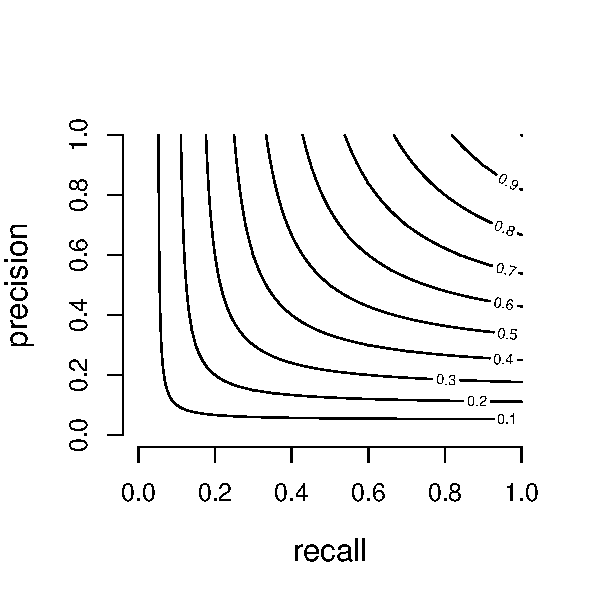
\includegraphics[height=2.5in]{pdfs/f-measure-contour.pdf}
\end{center}
\vspace*{-24pt}
\caption{Contour plot of $F$ measure as a function of recall and
  precision.  Each contour line indicates a particular $F$ measure
  value as marked.  For any given precision and recall, we can see
  roughly the result $F$ measure by which contour lines they're
  between.  For instance, tracing a line up from 0.4 recall to 0.6
  precision leaves us roughly equidistant between the $F=0.4$ and
  $F=0.5$ contour lines.}\label{fig:f-measure-contour}
\end{figure}


Although precision and recall are the most commonly reported pair of
statistics for natural language classification tasks, neither of them
involve the true negative count.  That is, they are only based on the
TP, FP and FN counts, which involve either a positive reference
category or positive response.



\subsection{The \code{PrecisionRecallEvaluation} Class}

The LignPipe class \code{PrecisionRecallEvaluation}, from the package
\code{com.aliasi.classify}, encapsulates a precision-recall matrix and
provides methods for the common statistics described in this section
as well as the confusion matrix methods detailed the previous section.  

\subsubsection{Construction and Population}

There are two constructors for a precision-recall evaluation instance.
The first, \code{PrecisionRecallEvaluation()}, starts with zero counts
in all cells, whereas
\code{PrecisionRecallEvaluation(long,long,long,long)} starts with the
specified number of TP, FN, FP, and TN counts respectively.

Once a precision-recall evaluation instance is constructed, the method
\code{addCase(boolean,boolean)} adds another test case, where the
first boolean argument represents the reference category and the
second the response category.  Positive responses are coded as boolean
\code{true} and negatives as \code{false}.  Thus calling
\code{addCase(true,true)} adds a true positive,
\code{addcase(true,false)} a false negative,
\code{addcase(false,false)} a true negative, and
\code{addcase(false,true)} a false positive.

\subsubsection{Counts and Statistics}

As for the confusion matrix implementation, the raw counts in the
cells as well as row- and column-wise sums are available directly.
The cell coutns are available through methods \code{truePositive()},
\code{falsePositive()}, \code{trueNegative()} and
\code{falseNegative()}.  

The basic statistics are also named in the obvious way, with the three
main methods being \code{precision()}, \code{recall()}, and
\code{fMeasure()}.  The precision-recall evaluation class ues the
terms \code{rejectionRecall()} for specificity and
\code{rejectionPrecision()} for selectivity, pointing out their
duality with precision and recall by swapping positive/negative
category naming.  

The row totals are availabe as \code{positiveReference()} and
\code{negativeReference()}, indicating the balance of positive and
negative cases in the reference (often the test) set.  Column totals
for responses are \code{positiveResponse()} and
\code{negativeResponse()}.  The total number of items, that is the
sum of all cells, is available through \code{total()}.

The proportion of positive cases in the reference set is given by
\code{referenceLikelihood()}, and the corresponding statistic for
responses, namely the proportion of positive responses, as
\code{responseLikelihood()}.  

All of the other statistics are defined in exactly the same way as for
consuion matrices.

\subsubsection{Demo: Precision-Recall Evaluations}

We provide a demo of precision-recall evaluations in the class
\code{PrecisionRecallDemo}.  We'll use the one-versus-all
classification matrix as we provided as a demo in
\reffig{blind-wine-one-versus-all}, which is the same as the result of
running the confusion matrix demo in
\refsec{classifier-eval-confusion-matrix-demo} and retrieving the
one-versus-all evaluation for cabernet.

All of the work's done in the \code{main()} method, which accepts four
arguments, representing the TP, FN, FP and TN counts respectively.
These are parsed as long values and assigned to variables \code{tp},
\code{fn}, \code{fp}, and \code{tn} respectively.  At this point,
we can construct our evaluation and inspect the counts assigned.
%
\codeblock{PrecisionRecallDemo.1}
%
We may then retrieve the various precision- and recall-like statistics
from the evaluation, including $F$ measure (and prevalence).
%
\codeblock{PrecisionRecallDemo.2}
%
Finally, we pull out some of the statistics that are available; the
rest are defined in the Javadoc and explained in the confusion matrix
demo.
%
\codeblock{PrecisionRecallDemo.3}

We can run the demo using the Ant target \code{precision-recall}.  It
provides the values of properties \code{tp}, \code{fn}, \code{fp}, and
\code{tn} as the first four arguments.  For instance, we can call it
with the values from the syrah-versus-all evaluation.
%
\commandlinefollow{ant -Dtp=9 -Dfn=3 -Dfp=4 -Dtn=11 precision-recall}
\begin{verbatim}
tpOut=9    fnOut=3    fpOut=4    tnOut=11
positiveRef=12    positiveResp=13    total=27
precision=0.692    recall=0.75    fMeasure=0.719
specificity=0.733    selectivity=0.785    prevalence=0.444
accuracy=0.740    accuracyStdDev=0.084
kappa=0.479    chisq=6.23
\end{verbatim}
%
We've reduced the number of digits by truncation and removed some
line breaks to save space in the book.


\section{Micro- and Macro-Averaged Statistics}

So far, in considering confusion matrices, we only considered overall
evaluation measures, such as accuracy, $\kappa$ statistics, and
$\chi^2$ independence tests.  In this section, we consider two 
ways of evaluating general classification results on a more
category-by-category basis.

\subsection{Macro-Averaged One Versus All}

In our treatment of confusion matrices, we showed how the $3 \times 3$
confusion matrix in \reffig{blind-wine-confusion} could be reduced the
three $2 \times 2$ confusion matrices, shown in
\reffig{blind-wine-one-versus-all}.

Suppose take each of these $2 \times 2$ confusion matrices and
consider its precision, recall and $F$ measure.  For instance,
precision for the cabernet matrix is approximately 0.69, for syrah
approximately 0.56, and for pinot noir 0.67.  The macro-averaged
precision is then given by averaging these values, the result of which
is 0.64.  We can similarly macro average any of the precision-recall
evaluation statistics.  Most commonly, we see macro-averaged values
for precision, recall, and $F$ measure.

Macro averaging has the property of emphasizing instances in low-count
categories more than in high-count categories.  For instance, even
though there are only 6 actual pinots versus 12 actual cabernets,
recall on the 6 pinots is weighted the same as recall on the 12
cabernets.  Thus the pinot recall is weighted twice as heavily
on a per-item basis.

Macro averaging is often used for evaluations of classifiers, with the
intent of weighting the categories equally so that systems can't spend
all their effort on high-frequency categories.


\subsection{Micro-Averaged One Versus All}

Micro-averaging is like macro-averaging, only instead of weighting
each category equally, we weight each item equally.  In practice, we
can compute micro-averaged results over the $2 \times 2$
precision-recall matrix produced by summing the three one-versus-all
precision-recall matrices.  We showed an example of this in
\reffig{blind-wine-micro}, which is the result of simply adding up the
three one-versus-all evaluations in
\reffig{blind-wine-one-versus-all}.

When we sum one-versus-all matrices, we wind up with a matrix with a
number of true positives equal to the number of elements on the
original matrix's diagonal.  That is, the true positives in the
micro-averaged matrix are just the correct answers in the original
matrix, each of which shows up as a true positive in exactly one of
the one-versus-all matrices (the one with its category).  

In the micro-averaged confusion example in \reffig{blind-wine-micro},
we have 18 true positives and 9 false positives, for a precision of
exactly 2/3.  Recall is also exactly 2/3.  And so is $F$ measure.  

Micro-averaged results are often reported along with macro-averaged
results for classifier evaluations.  If the evaluators care about
ranking classifiers, this provides more than one way to do it, and
different evaluatiosn focus on different measures.

\subsection{Demo: Micro- and Macro-Averaged Precision and Recall}

A demo for micro- and macro-averaged results is in the class
\code{MicroMacroAvg}.  The code is all in the \code{main()} method,
which expects no arguments.  It starts by setting up a confusion
matrix exactly as in our confusion matrix demo, so we don't show that.
The calculation of micro- and macro-averaged results is as follows.
%
\codeblock{MicroMacroAvg.1}
%
The macro-averaged results are computed directly by the confusion
matrix class.  The micro-averaged results are derived by first
extracting a precision-recall matrix for micro-averaged results,
then calling its methods.  

For convenience, we also extract all the precision-recall
evaluations on which the macro-averaged results were based and
extract their precision, recall and $F$ measures.
%
\codeblock{MicroMacroAvg.2}
%
We do not show the print statements.

The demo may be run from Ant using the target \code{micro-macro-avg}.
%
\commandlinefollow{ant micro-macro-avg}
\begin{verbatim}
cat=cabernet prec=0.692 rec=0.750 F=0.720
cat=   syrah prec=0.556 rec=0.556 F=0.556
cat=   pinot prec=0.800 rec=0.667 F=0.727
Macro prec=0.683 rec=0.657 F=0.668
Micro prec=0.667 rec=0.667 F=0.667
\end{verbatim}
%
From these results, it's also clear that we can recover the
micro-averaged results by taking a weighted average of the
one-versus-all results.  For instance, looking at recall, we have
one-versus-all values of 0.750 for cabernet, 0.556 for syrah, and
0.667 for pinot.  If we average these results weighted by
the number of instances (12 for cabernet, 9 for syrah, 6 for pinot),
we get the same result,
%
\begin{equation}
0.667 = \frac{(12 \times 0.750) + (9 \times 0.556) + (6 \times 0.667)}{12 + 9 + 6}.
\end{equation}
%
In most evaluations, micro-averaged results tend to be better, because
performance is usually better on high-count categories than low-count
ones.  Macro-averaged results will be higher than micro-averaged ones
if low count categories perform relatively better than high count
categories.

\subsection{Generalized Precision-Recall Evaluations for Information Extraction}

Precision-recall evaluations are applicable to broader classes of
problems than simple classifiers.  In fact, the most popular
applications of precision-recall evaluations are to
information-finding problems.  A typical example of this is named
entity mention recognition.  A named-entity mention is a sequence of
text that refers to some object in the real world by name.  For
example, \stringmention{Detroit} might refer to a city,
\stringmention{Denny McClain} to a person, and \stringmention{Tigers}
to an organization in the sentence \stringmention{Denny McClain played
  for the Tigers in Detroit}.

Suppose we have a reference corpus of named entity mentions.  We
evaluate a named-entity mention chunking system by running it over the
text and returning all the entity mentions found by the system.  Given
the reference answers, it's easy to classify each mention returned by
the system as a true positive if the response matches a mention in the
reference or a false positive if the response doesn't match a mention
in the reference.  Then, each mention in the reference that's not in
the response is marked as a false negative.  With the TP, FP, and FN
statistics, it's straightforward to compute precision and recall.

We have so far said nothing about true negatives.  The problem with
true negatives for a named entity mention finding task is that any
span of text may potentially refer to any type of entity, so there are
vast numbers of true negatives.  For instance, \stringmention{played},
\stringmention{McClain played}, \stringmention{played for},
\stringmention{McClain played for}, and so on, are all true negatives
in our example for any type of entity to which they're assigned.

This explains why precision is a more popular measure of information
extraction systems than specificity.  For specificity, we need to know
about the true negatives, whereas precision and recall are based only
on the combined set of positive reference items and positive response
items.

Similar precision-recall evaluations are applied to information
retrieval (IR) systems.  In the standard Cranfield evaluation model%
%
\footnote{Developed around the Cranfield test collection of 1400
documents in aeronautics in the 1960s.}
%
for evaluating IR systems, a test (or reference) corpus consists of a
sequence of queries and for each query, the set of relevant documents
from a collection.  A system then returns a number of documents for a
query.  Each of these returned document will be either a true positive
(if it's marked as relevant in the reference corpus) or a false
positive (if it's not marked as relevant).  The relevant documents not
returned are false negatives and the rest are true negatives.  These
evaluations are often extended to systems that provide ranked and
scored results, as we discuss in the next section.


\section{Scored Precision-Recall Evaluations}

So far, we have assumed that the system's response to a classification
problem is a single first-best guess at a category.  Many different
kinds of classifiers support returning more than one guess, typically
with a score for each result determining a rank order.  In many cases,
the results are associated with conditional probability estimates of
the response category given the item being classified; in other cases,
scores have a geometric interpretation, such as the margin from the
classification hyperplane for a perceptron or the cosine for TF/IDF
rankings.


\subsection{Ranks, Scores and Conditional Probability Estimates}

For instance, given our blind-wine grape-guessing task, a taster may
be presented with a wine, and respond that their first guess is
cabernet, their second guess syrah, and their third guess pinot noir.
That's a ranked response.  In addition, they might further specify
that cabernet has a score of $-1.2$, syrah a score of $-1.3$, and
pinot a score of $-2.0$ (yes, scores may be negative; they still get
sorted from largest, here $-1.2$, to smallest, $-2.0$, for
purposes of ranking).  That's what we call a scored response.  

An even more refined response contains a conditional probability
estimate of the output category given the input, such as 55\%
cabernet, 35\% syrah, and 10\% pinot noir.  That's a conditional
probability response.%
%
\footnote{There are also joint probability responses, from which
  conditional probabilities can be derived.  The joint probabilities
  are less useful for evaluation, so we put off considering them until
  we see a classifier that uses them.}

\subsection{Comparing Scores across Items}

Ranked results support ranking categories within the response to a
single item being classified, such as a single wine.  For instance, I
may be guessing the grapes in two wines, and rank the first one syrah,
cabernet, and pinot, and the second one pinot, syrah, and cabernet.
Without scores, there's no way to tell if the taster is more confident
about the guess of syrah for the first wine or pinot for the second
wine.

With scores, we are sometimes able to compare a classifier's response
across items.  Usually we can't, though, because the scores will only
be calibrated among the category responses for a single item.  For
instance, it doesn't usually make sense to compare scores for
different documents across different searches in an information
retrieval system like Lucene (see \refchap{lucene}), because of all
the document- and query-specific effects built into scoring.

Conditional probabilities, on the other hand, are naturally calibrated
to be comparable across runs.  If I have two wines, and for the first
one respond 55\% cabernet, 35\% syrah and 10\% pinot, and for the
second, 90\% cabernet, 8\% syrah, and 2\% pinot, I can rank my
choices.  My best guess is that wine 2 is a cabernet, because I've
estimated a 90\% chance of being right.  My second best guess is that
wine 1 is a cabernet (55\%), my third-best guess that wine 1 is a
syrah (35\%), my fourth-best guess that wine 1 is pinot (10\%), my
fifth-best that wine 2 is syrah (8\%), and my least likely guess is
that wine 2 is a pinot (2\%).

In this section, we will assume that we're evaluating system responses
in a situation where the scores (or conditional probabilities) are
calibrated across different items.  This lets us arrange all of our
guesses for all of our items in order.  It is this ordering, an example
of which we saw in the last paragraph, that forms the basis for
scored precision recall evaluations.

\subsection{The \code{ScoredPrecisionRecallEvaluation} Class}

The LingPipe class \code{ScoredPrecisionRecallEvaluation}, in package
\code{com.aliasi.classify}, implements precision-recall type
statistics based on scored results.  

\subsubsection{Construction and Population}

Most often, like precision-recall evaluations, scored precision-recall
evaluations will be constructed automatically by encapsulated testing
classes for each kind of system.  LingPipe generates scored
precision-recall evaluations when given appropriately probabilistic
taggers, chunkers, spelling correctors, or classifiers.  For now, we
consider direct construction and manipulation to get a feeling for the
evaluation class itself.

There is a single no-arg constructor,
\code{ScoredPrecisionRecallEvaluation()}.  The evaluation initially
starts out with no data.

Responses are added to the evaluation using the method
\code{addCase(boolean,double)}, which takes two arguments, the first
being whether the result was correct, and second what the score was.
Note that we are not keeping track of the individual categories, just
their scores and whether they are correct or not.

Going back to our example, of the previous section, suppose the first
wine was a syrah, and the second a cabernet.  Here we repeat the
responses along with an indication of whether the response was true or
not.  For the first wine, we have 55\% cabernet (false), 35\% syrah
(true), and 10\% pinot noir (false), and for the second wine, 90\%
cabernet (true), 8\% syrah (false), and 2\% pinot noir (false).  To
populate the evaluation with these results requires six calls to
\code{addCase()}, \code{addCase(false,0.55)},
\code{addCase(true,0.35)}, and \code{addCase(false,0.10)} for the three
responses for the first wine, and similarly for the three results from
the second wine.

If the responses are exhaustive for each item, this is all we have to
do.  The key observation is that the correct answers will show up in
every set of responses.  Unfortunately, this is often not the case.
For instance, consider a named-entity chunker that returns the
100-best potential entity mentions for each sentence.  If we know the
true entity mentions, we can rank each of these results as true or
false, based on whether the entity mention is in the reference
standard or not.  But there's no guarantee that the system will find
all the entities in a sentence, even if it returns its 100-best
guesses.

In the case where not every positive reference item is included in the
system response, the method \code{addMisses(int)} lets you add in the
number of positive reference items that were missed by the system's
responses.  For instance, suppose we have the following sentence, marked
for named entities.
%
\begin{verbatim}
Johan van der Dorp took the train to den Haag.
01234567890123456789012345678901234567890123456
0         1         2         3         4
(0,18):PER   (37,45):LOC
\end{verbatim}
%
The entities are marked by character offsets, with \code{(0,18):PER}
indicating that the text spanning from character 0 (inclusive) to
character 18 (exclusive), namely \stringmention{Johan van der Dorp},
mentions a person.  Simiarly, the other entity indicates that
\stringmention{den Haag} refers to a location.  This is a tricky
sentence for a system trained on English data without an extensive
list of names or locations, because both names contain tokens that are
not capitalized.  

Given the input text, a named-entity mention chunker might return all
found chunks with estimated probability above 0.01, which might lead
to the following six chunks, for example.
%
\begin{verbatim}
( 4, 8):LOC  0.89     (41,45):ORG  0.43     (41,45):LOC  0.09
( 0, 5):PER  0.46     (41,45):PER  0.21     ( 0,18):PER  0.02
\end{verbatim}
%
In this case, only the guess \code{(0,18):PER} is correct, with the
other five being wrong.  We call \code{addScore()} for each response,
including the probability estimate and correctness, the latter of
which is false for the first five responses and true for the last one.
After adding the scores, we must call \code{addMisses(1)}, indicating
that one of the reference entities, namely \code{(37,45):LOC}, was not
included among the system responses.%
%
\footnote{These low-level adds, for both found chunks and misses, is
  automated in the chunker evaluation classes.  We're just using named
  entity spotting as an example here.}

To evaluate information retrieval results, the system is used in the
same way, with the method \code{addScore()} being called for each
system response and \code{addMisses()} for the results that the
system didn't return.


\subsection{Demo: Scored Precision-Recall}

We provide a demo of the scored precision-recall evaluation class in
\code{ScoredPrecisionRecallDemo}.  All of the work is in the
\code{main()} method, which has no command-line arguments.

\subsubsection{Construction and Population of Results}

The \code{main()} method starts by constructing an evaluation and
populating it.
%
\codeblock{ScoredPrecisionRecallDemo.1}
%
After construction, we add ten scored results, four of which are true
positives and six of which are false positivies.  We then add a
single miss representing a reference positive that was not returned by
the system.

\subsubsection{Statistics at Ranks}

The evaluation is most easily understood by considering the sorted
table of evaluated responses, which may be found in
\reffig{scored-pr-example}.
%
\begin{figure}
\begin{center}
\begin{tabular}{rrcccccccc}
\tblhead{Rank} & \tblhead{Score} & \tblhead{Correct} & \tblhead{TP} & \tblhead{TN} & \tblhead{FP} & \tblhead{FN} 
  & \tblhead{Rec} & \tblhead{Prec} & \tblhead{Spec}
\\ \hline
0 & $-1.21$ & no & 0 & 5 & 1 & 5 & 0.00   & 1.00   & 0.83
\\
1 & $-1.27$ & {\bf yes} & 1 & 5 & 1 & 4 & {0.20}  & 0.50  & {0.83}
\\
2 & $-1.39$ & no  & 1 & 4 & 2 & 4 & 0.20  & 0.33  & 0.67
\\
3 & $-1.47$ & {\bf yes} & 2 & 4 & 2 & 3 & {0.40}  & 0.50  & 0.67
\\
4 & $-1.60$ & {\bf yes} & 3 & 4 & 2 & 2 & {0.60}  & {0.60}  & {0.67}
\\
5 & $-1.65$ & no & 3 & 3 & 3 & 2 & 0.60  & 0.50  & 0.50
\\
6 & $-1.79$ & no & 3 & 2 & 4 & 2 & 0.60  & 0.43  & 0.33
\\
7 & $-1.80$ & no & 3 & 1 & 5 & 2 & 0.60  & 0.38  & 0.17
\\
8 & $-2.01$ & {\bf yes} & 4 & 1 & 5 & 1 & {0.80}  & {0.44}  & {0.17}
\\
9 & $-3.70$ & no & 4 & 0 & 6 & 1 & 0.80  & 0.40  & 0.00
\\ \hline
10 & miss & {\bf yes} & 5 & 0 & 6 & 0 & 1.00 & 0.00 & 0.00
\end{tabular}
\vspace*{-8pt}
\end{center}
\caption{Example of a scored precision-recall evaluation.  The
  responses are shown with their correctness, sorted by score.  There
  is a single missed positive item for which there was no response, so
  we include it at the bottom of the table without a score.  In total,
  the number of positive cases is 5 and the total number of negative
  cases is 5.  The ranks, numbered from 0, are determined by score.
  The counts of TP, TN, FP and FN and the corresponding recall
  $(\mbox{TP}/(\mbox{TP}+\mbox{FN}))$, precision
  $(\mbox{TP}/(\mbox{TP}+\mbox{FP}))$, and specificity
  $(\mbox{TN}/(\mbox{TN}+\mbox{FP}))$ values are
  shown.}\label{fig:scored-pr-example}
\end{figure}
%
The first column of the table indicates the rank of the response
(numbering from zero), the second the score of the response, and the
third whether it was a correct (true) response or not.  For example,
the top-ranked response has a score of $-1.21$ and is incorrect,
whereas the second-best response has a score of $-1.27$ and is correct.

We use this table to generate confusion matrices for precision/recall for
all of the results up to that rank.  The next four columns represent
the counts in the cells of the confusion matrix, TP, TN, FP,
and FN, for each rank.  These are the basis for the computation of the
next three columns, which are recall, precision, and specificity, at
rank $N$.%
%
\footnote{LingPipe numbers ranks from zero for the purpose of
  precision-recall and ROC curves, but numbers them from one for the
  purposes of computing the conventional precision-at-rank and
  reciprocal rank statistics.}
%
For recall, this is the fraction of all reference positive items that
have been retrieved at the specified rank or before.  The highest
recall achieved for non-zero precision is only 0.80 because we added
a missed item, for a total of five reference positive items.  Every
time we hit a correct answer, the recall (sensitivity) and precision
go up and specificity stays the same.

Precision is calculated slightly differently, being the fraction of
results returned so far that are correct.  Thus the first value is
zero, because we have $\mbox{TP}=0$ and $\mbox{FP}=1$ at this point,
for a precision of $\mbox{TP}/(\mbox{TP}+\mbox{FP}) = 0$.  At rank 1,
we have $\mbox{TP}=1$ and $\mbox{FP}=1$, for a precision of 0.5.  By
the time we get down to rank 9, we have $\mbox{TP}=4$ and
$\mbox{FP}=6$, for a precision of 0.4.  We pin the precision and
specificity of results corresponding to calls to \code{addMisses()} to
0, because there is no indication of the number of false positives
that may show up ahead of the misses.

Specificity (or rejection recall) is calculated more like recall than
precision.  Specifically, we assume that at each rank, we have
correctly rejected all the items we haven't mentioned.  So at rank 0,
we have $\mbox{TN} = 6$ and $\mbox{FP}=1$.

\subsubsection{Inspecting Precision-Recall Curves}

After constructing and populating the evaluation, the code in the
\code{main()} method goes on to print out the precision-recall curve
implied by the data and represented in the instance \code{eval} of
a scored precision-recall evaluation.
%
\codeblock{ScoredPrecisionRecallDemo.2}
%
We have set the interpolation flag to false, and then walked over the
resulting curve pulling out recall/precision operating points (and
then printing them in code not shown).  

The Ant target \code{scored-precision-recall} runs the demo, which
takes no command-line arguments.  If we run it, the following shows
the results for uninterpolated and interpolated precision-recall
curves (the repeated code to print out the interpolated results
is not shown here; it only differs in setting the interpolation
flag to \code{true}).
%
\commandlinefollow{ant scored-precision-recall}
\begin{verbatim}
Uninterpolated P/R     Interpolated P/R
prec=1.00 rec=0.00     prec=1.00 rec=0.00
prec=0.50 rec=0.20     prec=0.60 rec=0.20
prec=0.33 rec=0.20     prec=0.60 rec=0.40
prec=0.50 rec=0.40     prec=0.60 rec=0.60
prec=0.60 rec=0.60     prec=0.44 rec=0.80
prec=0.50 rec=0.60     prec=0.00 rec=1.00
prec=0.43 rec=0.60
prec=0.38 rec=0.60
prec=0.44 rec=0.80
prec=0.40 rec=0.80
prec=0.00 rec=1.00
\end{verbatim}
%
The uninterpolated results are just the precision and recall values
from our table.  Interpolation has the effect of setting the precision
at a given recall point $r$ to be the maximum precision at any
operating point of the same or higher recall.  For instance, the
precision at recall point 0.4 is interpolated to 0.6, becaus ethe
precision at recall point 0.6 is 0.6.

A graph of the uninterpolated and interpolated precision-recall
curves are shown in \reffig{pr-curves}.
%
\begin{figure}
\begin{center}
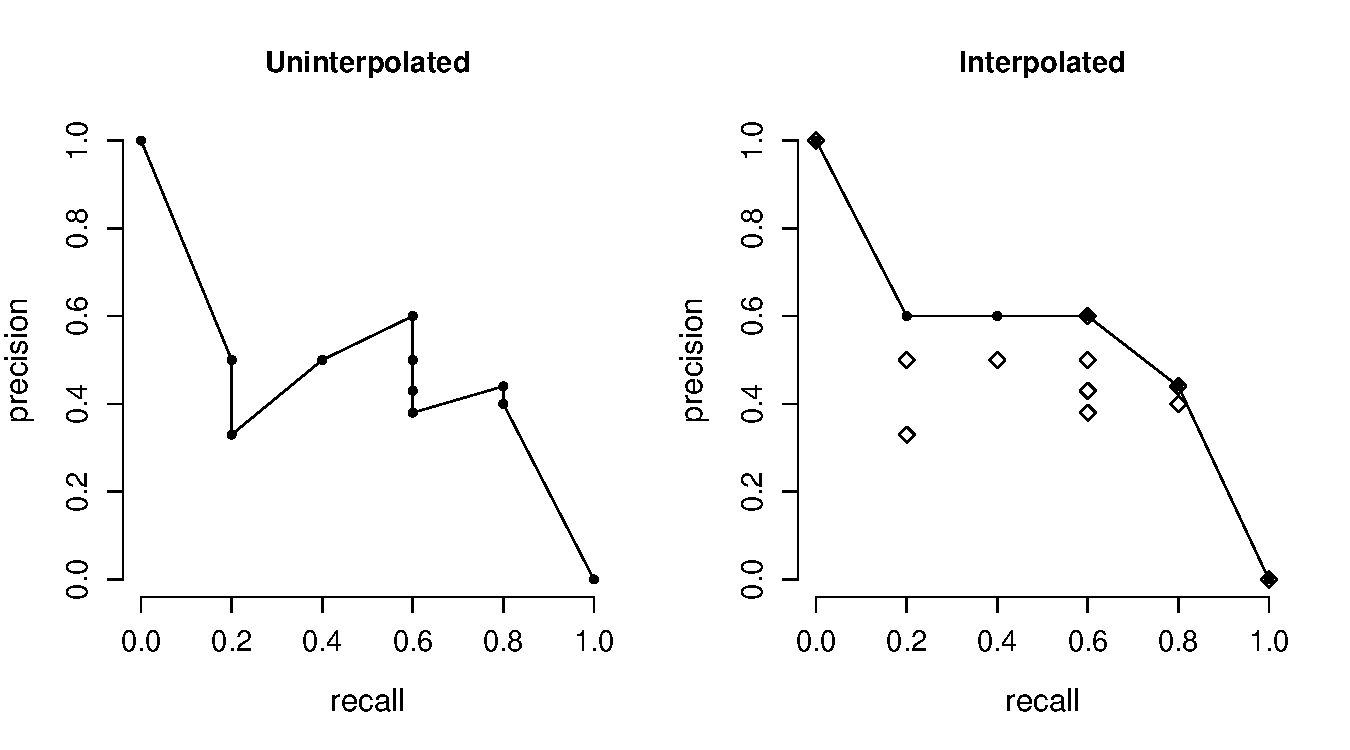
\includegraphics[height=2.5in]{pdfs/pr-curves.pdf}
\vspace*{-24pt}
\end{center}
\caption{Uninterpolated and interpolated precision-recall curves
  for the data in \reffig{scored-pr-example}.  In both graphs, the filled
  circles are the points on the curve.  In the interpolated graphs,
  the diamonds correspond to points on the original, uninterpolated,
  curve.}\label{fig:pr-curves}
\end{figure}


\subsubsection{Inspecting ROC Curves}

The code for retrieving receiver operating characteristic (ROC) curves
is identical to that for precision/recall curves, only it uses the
method \code{rocCurve(boolean)} rather than \code{prCurve(boolean)}
and returns $1-\mbox{specificity}$/sensitivity pairs instead of
recall/precision pairs.
%
\codeblock{ScoredPrecisionRecallDemo.3}
%
The output from this block of code, and from the next block, which is
identical other than setting the interpolation flag, is as follows.
%
\begin{verbatim}
Uninterpolated ROC        Interpolated ROC
1-spec=0.00 sens=0.00     1-spec=0.00 sens=0.00
1-spec=0.17 sens=0.00     1-spec=0.17 sens=0.20
1-spec=0.17 sens=0.20     1-spec=0.33 sens=0.60
1-spec=0.33 sens=0.20     1-spec=0.50 sens=0.60
1-spec=0.33 sens=0.40     1-spec=0.67 sens=0.60
1-spec=0.33 sens=0.60     1-spec=0.83 sens=0.80
1-spec=0.50 sens=0.60     1-spec=1.00 sens=1.00
1-spec=0.67 sens=0.60
1-spec=0.83 sens=0.60
1-spec=0.83 sens=0.80
1-spec=1.00 sens=0.80
1-spec=1.00 sens=1.00
\end{verbatim}
%
Interpolation works the same way as for precision-recall curves,
removing dominated points with the same $x$-axis value.  
Graphs of the uninterpolated and interpolated ROC curves are shown in 
\reffig{roc-curves}.
%
\begin{figure}
\begin{center}
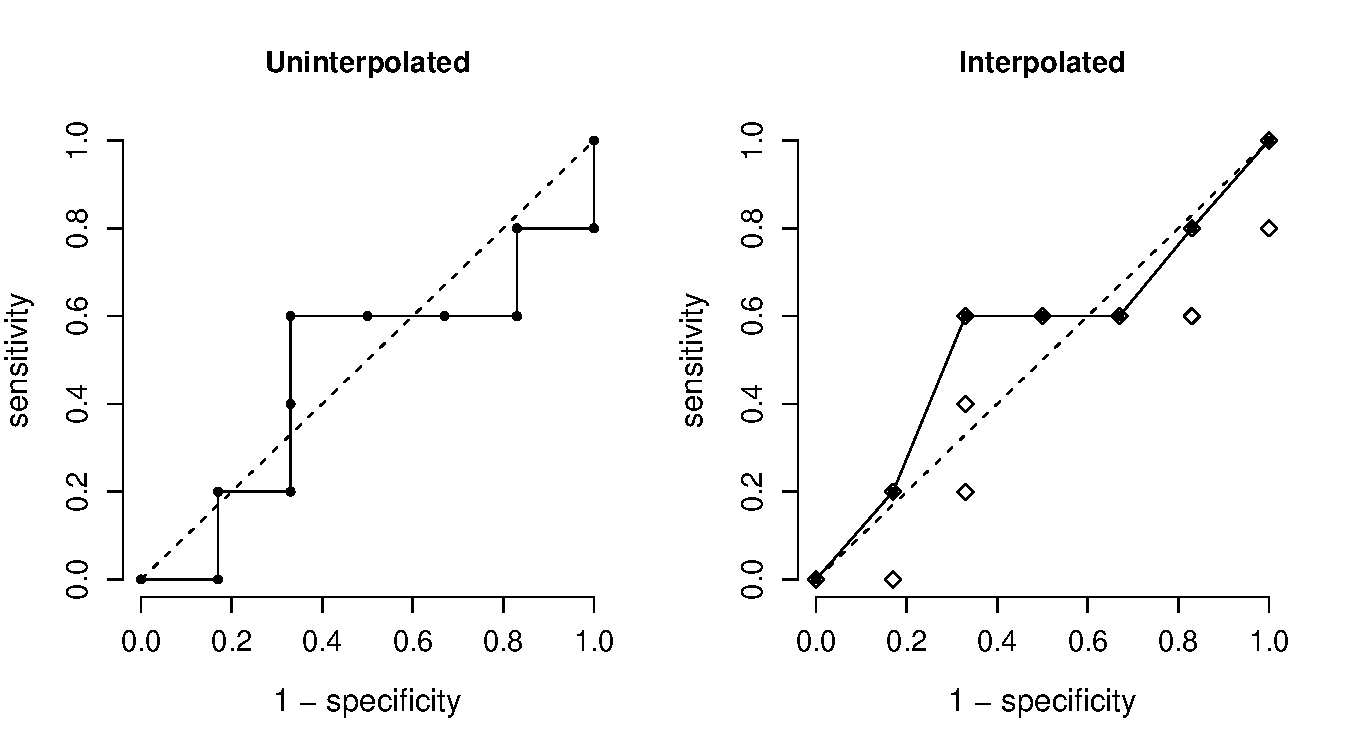
\includegraphics[height=2.5in]{pdfs/roc-curves.pdf}
\vspace*{-24pt}
\end{center}
\caption{Uninterpolated and interpolated receiver-operating
  characteristic curves for the data in \reffig{scored-pr-example}.  In
  both graphs, the filled circles are the points on the curve.  In the
  interpolated graph, the diamonds correspond to points on the
  original, uninterpolated, curve.  The dashed diagonal line is
  at chance performance.}\label{fig:roc-curves}
\end{figure}



The method \code{addNegativeMisses(int)} adds to the overall count of
reference negative items.  Because these will all be correctly
rejected by not being returned, adding negative misses will primarily
boost the specificity in ROC cuves.  

We believe the precision-recall and ROC curves provide the best view
of how a classifier works.  It shows how tradeoffs may be made between
precision and recall by setting different operating points for
accepting a result.  It is important to keep in mind, though, that
these results are on evaluation data, and represent only an estimate
of what results will be on unseen data.  In practice, if results were
achieved through tuning by cross validation, the precision-recall and
ROC curves will be overly optimistic.


\subsubsection{$F$ Measure at Rank}

LingPipe only returns the precision-recall operating points, not the
$F$ measure.  To compute $F$ measure, the static utility method
\code{fMeasure(double,double,double)} may be used to compute the $F$
measure of any two operating points.  The three arguments are for the
precision weight (which should be 1 as we have defined $F$ measure
here; see the next section for generalizations), and for precision and
recall (though the order of precision and recall doesn't matter for
computing $F$ measure). So the call looks like
\code{fMeasure(1.0,p,r)}, where the \code{1.0} just indicates that
precision and recall are balanced, \code{p} is precision, and \code{r}
is recall.

\subsubsection{Precision at Rank $N$}

For scored precision-recall evaluations, the method
\code{precisionAt(int)} returns the precision at a specified rank.
For example, with the data in \reffig{scored-pr-example}, the
precision at rank $N$ is determined by looking up the precision for
that rank.  Ranks are conventionally counted from 1, so that is how we
count for the \code{precisionAt()} method.

The precision at every rank is calculated with the following code.
%
\codeblock{ScoredPrecisionRecallDemo.4}
%
Note that our loop starts from 1 and uses a less-than-or-equal bound
test to adjust for the fact that precision-at ranks start at 1.  The
output corresponds to the precisions in \reffig{scored-pr-example}.
%
\begin{verbatim}
Prec at  1=0.00     Prec at  5=0.60     Prec at  9=0.44
Prec at  2=0.50     Prec at  6=0.50     Prec at 10=0.40
Prec at  3=0.33     Prec at  7=0.43     Prec at 11=0.36
Prec at  4=0.50     Prec at  8=0.38
\end{verbatim}
%

\subsubsection{Maximum $F$ Measure and BEP}

Two other commonly reported operating points derived from the
precision-recall curve are the maximum $F$ measure and
precision-recall breakeven point (BEP).  Continuing our example,
these are extracted as follows.
%
\codeblock{ScoredPrecisionRecallDemo.5}
%
Their values are output (code not shown) as 
\begin{verbatim}
Maximum F =0.60      Prec/Rec BEP=0.44
\end{verbatim}

These values are both computed from the uninterpolated curves and
correspond to real points on the operating curve.

Break-even point is also known as $R$-precision, because it is
equivalent to the precision at $R$, where $R$ is the number of
reference positive results.  That's because if we have $n$ true
positives after $R$ results, the the precision and recall are both
$n/R$.



\section{Contingency Tables and Derived Statistics}\label{section:classifier-eval-contingency-table}

In this section, we provide a precise definition of contingency tables
and discuss the computation and interpretation of statistics on
contingency tables.  

A contingency table is an $M \times N$ matrix $C$ of counts
\ie{$C_{m,n} \in \nats$}.  A generic contingency table is shown in
\reffig{stats-generic-contingency-table}.
%
\begin{figure}
\begin{center}
\begin{tabular}{c|cccc||c}
& 1 & 2 & $\cdots$ & $N$ & \tblhead{Total}
\\ \hline
1 & $C_{1,1}$ & $C_{1,2}$ & $\cdots$ & $C_{1,N}$ & $C_{1,+}$
\\
2 & $C_{2,1}$ & $C_{2,2}$ & $\cdots$ &  $C_{2,N}$ & $C_{2,+}$
\\
$\vdots$ & $\vdots$ & $\vdots$ & $\ddots$ & $\vdots$ & $\vdots$
\\
$M$ & $C_{M,1}$ & $C_{M,2}$ & $\cdots$ & $C_{M,N}$ & $C_{M,+}$
\\
\hline \hline
\tblhead{Total} & $C_{+,1}$ & $C_{+,2}$ & $\cdots$ & $C_{+,N}$& $C_{+,+}$
\end{tabular}
\end{center}
\vspace*{-12pt}
\caption{A generic $M \times N$ contingency table $C$.  Each entry
  $C_{m,n}$ represents a cell count.  The values along the bottom and
  on the right side are totals of their respective columns and rows.
  The value in the lower right corner is the total count in the
  table.}\label{fig:stats-generic-contingency-table}
\end{figure}
%
We use the notation $C_{m,+}$ for the sum of the values in row $m$,
$C_{+,n}$ for the sum of the values in column $n$, and and $C_{+,+}$
for the sum of the entire table.  These values are defined by
%
\begin{equation}
C_{m,+} = \sum_{n=1}^N C_{m,n}, 
\ \ \ \ \ \
C_{+,n} = \sum_{m=1}^M C_{m,n}, \mbox{ and}
\ \ \ \ \ \  
C_{+,+} = \sum_{m=1}^M \sum_{n=1}^N C_{m,n}.
\end{equation}



\subsection{$\chi^2$ Tests of Independence}\label{section:stats-chi-square-independence}

The $\chi^2$ distribution may be used to test the null hypothesis that
that a pair of categorical random variables are generated
independently.

Suppose we have $K$ independent and identically distributed (i.i.d.)
pairs $A_k, B_k$ of categorical random variables taking values $A_k
\in 1{:}M$ and $B_k \in 1{:}N$.  Being identically distributed means
the pairs share distributions, so that
%
\begin{equation}
p\!_{A_i,B_i} = p\!_{A_j,B_j} \mbox{ for } i, j \in 1{:}K.
\end{equation}
%
Independence requires that the value of the pair $A_i,B_i$ is
independent of the value of the pair $A_j,B_j$ if $i \neq j$.

So far, we have allowed for the possibility that $A$ and $B$ are not
independent of each other.  If $A_k$ and $B_k$ are independent, then
%
\begin{equation}
p\!_{A_k,B_k}(x,y) = p\!_{A_k}(x) \times p_{B_k}(y).
\end{equation}
%
Because we've assumed the $A_k,B_k$ pairs are i.i.d., they share
distributions and hence are either all independent or all
non-independent.

We define an $M \times N$ contingency table $C$ by setting
%
\begin{equation}
C_{m,n} = \sum_{k=1}^K \indicator{A_k = m, B_k = n}.
\end{equation}
%
That is, $C_{m,n}$ is the number of times $A_i$ was $m$ and $B_i$ was
$n$.  Note that $C$ is a matrix random variable defined as a function
of the random variables $A$ and $B$.

Given a contingency table $C$, we can estimate the marginal
distributions $p_A(m)$ and $p_B(n)$ by maximum likelihood using the
observed counts in $C$.  Because $p_A$ and $p_B$ are multinomials, we
assume $p_A = \dbern{\theta}$ and $p_B = \dbern{\phi}$.  The
maximum likelihood estimates $\theta^*, \phi^*$ of $\theta,\phi$
given $C$ are
%
\begin{equation}
\theta^*_m = \frac{C_{m,+}}{C_{+,+}} 
\ \ \ \ \ \mbox{and} \ \ \ \ \ 
\phi^*_n = \frac{C_{+,n}}{C_{+,+}}.
\end{equation}

Pearson's independence test involves the statistic $X^2$, which is
defined in terms of $C$ by
%
\begin{equation}
X^2 
= \sum_{m=1}^M \ \sum_{n=1}^N 
  \frac{(C_{m,n} - E_{m,n})^2}
       {E_{m,n}}
\end{equation}
%
where $E_{m,n}$ is the expected value of $C_{m,n}$ (given our
estimates $\theta^*$ and $\phi^*$) if $A$ and $B$ are independent,
%
\begin{equation}
E_{m,n} = C_{+,+} \ \times \ \theta^*_m \ \times \ \phi^*_n.
\end{equation}

If $A_k$ and $B_k$ are independent, the distribution of the statistic
$X^2$ is approximately $\chi^2$ with $(M-1) \times (N-1)$ degrees of
freedom (see \refsec{stats-chi-squared-distribution}).%
%
\footnote{The proof is too complex, but we provide some hints as to
  its form.  We have $MN$ cells, so have $MN-1$ degrees of freedom, of
  which we lose $M-1$ and $N-1$ because we are estimating $\theta^*$
  and $\phi^*$, which have one less than their dimensionality degrees
  of freedom, $M-1$ and $N-1$, for a total of $MN-1 - (M + N -2) =
  (M-1)(N-1)$ degrees of freedom (again, asymptotically).  Because the
  $C_{m,n}$ are binomially distributed with success probability
  $\theta^*_m \times \phi^*_n$ and $C_{+,+}$ trials, the central limit
  theorem ensures asymptotic normality of $C_{m,n}$ as $C_{+,+}$
  grows.  The mean or expected value of the binomial is $E_{m,n}$, and
  a binomial's variance is equal to its mean.  Rewriting the term
  inside the summation in the definition of the $X^2$ statistic as
  $((C_{m,n} - E_{m,n})/\sqrt{E_{m,n}})^2$ reveals that its just a
  squared z-score.}
%
The usual rule of thumb is that the approximation is reliable if each
of the expected counts $E_{m,n}$ is at least 5.

As usual, the classical hypothesis test rejects the null hypothesis with
$p$-value $\alpha$ if the value of the test statistic $X^2$ is outside
of the central and columns are independent if the $X^2$ statistic is
outside of the central probabiilty interval of $1-p$.

\subsection{Further Contingency and Association Statistics}\label{section:classifier-eval-further-assoc}

\subsubsection{Pearson's Mean Square Contingency}

Dividing Pearson's $\chi^2$ statistic $X^2$ by the number of cases
yields Pearson's $\varphi^2$ statistic.
%
\begin{equation}
\varphi^2 =\frac{X^2}{C_{+,+}}
\end{equation}
%
The $\varphi^2$ statistic is known as the mean square contingency for
the table $C$.  As with $X^2$, larger values indicate more contingency.

\subsubsection{Cramér's Degree of Association}

Cramér's V statistic%
%
\footnote{H. Cramér. 1999. {\it Mathematical Methods of
    Statistics}. Princeton University Press.}
%
is designed to measure the degree of association between the
rows and columns in a general contingency table.   The square of
$V$ is defined by dividing $\varphi^2$ by the minimum of the number
of rows and columns minus 1,
%
\begin{equation}
V^2 = \frac{\varphi^2}{\min(M,N)-1}.
\end{equation}
%
Obviously, the definition only makes sense if $M,N \geq 2$, and if
$M=2$ or $N=2$, $V^2$ reduces to $\varphi^2$.  As with $\varphi^2$ and
$X^2$, larger values of $V^2$ indicate stronger associations.

\subsubsection{Goodman And Kruskal's Index of Predictive Association}

Goodman and Kruskal defined an asymmetric measure of predictive
association which they called $\lambda_B$.%
%
\footnote{Goodman and Kruskal wrote three papers analyzing
  cross-classified data such as is found in contingency matrices,
  starting with Goodman, L.~A. and W.~H.~Kruskal, 1954, Measures of
  association for cross classifications, Part I, {\it Journal of the
    American Statistical Association} {\bf 49}:732–-764.  With the
  same journal and title, Part II was
  published in 1959 in volume {\bf 53}, pages 123--163, and Part III
  in 1963 in volumne {\bf 58}, pages 310--364.}
%
The value of $\lambda_B$ is (an estimate of) the reduction in error
likelihood from knowing the response category and using it to predict
the reference category.  It takes on values between 0 and 1, with
higher values being better, 0 indicating independence and 1 perfect
assocaition.  

Given our $M \times N$ confusion matrix $C$, Goodman and Kruskal's
index of predictive association $\lambda_B$ is defined by
%
\begin{equation}
\lambda_A 
= \frac{\left(\sum_n R_n\right) - S}
       {C_{+,+} - S}
\end{equation}
%
where $S$ and $R_n$ are defined by 
%
\begin{equation}
S = \max_n \ C_{+,n}
\ \ \ \ \ \mbox{and} \ \ \ \ \
R_n = \max_m \ C_{n,m}.
\end{equation}
%
These statistics are unusual in using the maximum rather than
matching.  Dividing through by $C_{+,+}$ reveals a structure very much
like the $\kappa$ statistic (see \refsec{stats-kappa}), with $e$
replaced by $S/C_{+,+}$ and with $a$ replaced by $\sum_n R_n /
C_{+,+}$.

The $\lambda_B$ statistic is not symmetric between the rows and
columns.  If we transpose the matrix and compute the same statistic,
we get $\lambda_Ap$.


\subsection{Information-Theoretic Measures}

If we use the counts in $C$ to estimate probability distributions
using maximum likelihood, we may use any of the information-theoretic
measures available to compare distributions (see
\refsec{stats-information-theory} for definitions).  

For example, suppose we define random variables $X$ and $Y$ for the
rows and columns, with joint distribution given by the maximum
likelihood estimate given the contingency table $C$, which entails
%
\begin{equation}
p_{X,Y}(m,n) = \frac{C_{m,n}}{C_{+,+}}.
\end{equation}
%
Given this defintion, the marginal distributions for $X$ and $Y$ are
%
\begin{equation}
p_X(m) = \frac{C_{m,+}}{C_{+,+}}
\ \ \ \ \ \mbox{and} \ \ \ \ \
p_Y(n) = \frac{C_{+,n}}{C_{+,+}}.
\end{equation}
%
The conditional distributions for $X$ given $Y$ and vice-versa are
%
\begin{equation}
p_{X|Y}(m|n) = \frac{C_{m,n}}{C_{m,+}}
\ \ \ \ \ \mbox{and} \ \ \ \ \
p_{Y|X}(m|n) = \frac{C_{m,n}}{C_{+,n}}.
\end{equation}

With all of these definitions in hand, we can easily compute the
various information theoretic measures, which are defined in
\refsec{stats-information-theory}.

For instance, we can compute the entropy corresponding to the rows of
the contingency table as $\entropy{X}$ and to the columns as
$\entropy{Y}$.  We can also compute the KL-divergences, symmetrized
divergences and Jensen-Shannon divergence based on the marginal
distributions $p_X$ and $p_Y$ implied by the contingency table.

With the joint and conditional estimates, we can tabulate the joint
entropy $\entropy{X,Y}$, conditional entropies $\condentropy{X}{Y}$
and $\condentropy{Y}{X}$, as well as and mutual information
$\mutualinfo{X}{Y}$.


\subsection{Confusion Matrices}

A confusion matrix is just a square ($N \times N$) contingency table
where the variable represented by the rows and columns has the same
set of categorical outcomes.  Confusion matrices are often used to
evaluate classifiers, taking the rows to represent reference
categories and columns to represent system responses.

There is a wide range of statistics that have been applied to
evaluating the performance of classifiers using confusion matrices.

\subsection{$\kappa$ Statistics for Chance-Adjusted Agreement}\label{section:stats-kappa}

Suppose we have an $N \times N$ confusion matrix $C$.  

Cohen's $\kappa$ statistic%
\footnote{Cohen, Jacob. 1960. A coefficient of agreement for nominal
  scales. {\it Educational And Psychological Measurement} {\bf
    20}:37-46.}
%
is defined by
%
\begin{equation}
\kappa = \frac{a - e}{1 - e},
\end{equation}
%
where
%
\begin{equation}
a = \frac{\sum_{n=1}^N C_{n,n}}{C_{+,+}}
\ \ \mbox{ and } \ \ 
e = \sum_{n=1}^N \theta^*_n \ \times \ \phi^*_n = \frac{E_{n,n}}{C_{+,+}}.
\end{equation}
%
In words, $a$ is the percentage of cases in which there was agreement,
in other words the total accuracy, and $e$ is the expected accuracy if
the reference and response are independent.

Siegel and Castellan's $\kappa$ statistic%
\footnote{Siegel, Sidney and N.~John Castellan, Jr. 1988.  {\it
    Nonparametric Statistics for the Behavioral Sciences}. McGraw
  Hill.}
%
has the same definitional form as Cohen's, but the calculation of the
expectation is based on averaging the reference and response to define
%
\begin{equation}
e = \sum_{n=1}^N \left( \frac{\theta^*_n + \phi^*_n}{2} \right)^2.
\end{equation}

Byrt et al.'s $\kappa$ statistic%
%
\footnote{Byrt, Ted, Janet Bishop and John B. Carlin. 1993. Bias,
  prevalence, and kappa. {\it Journal of Clinical Epidemiology}
  {\bf 46}(5):423--429.}
%
completely ignores the adjustment for
category prevalence found in $e$, taking an arbitrary 50\% chance of
agreement, corresponding to $e=1/2$, and resulting in a definition of
$\kappa = 2a - 1$.



\subsection{Sensitivity-Specificity Matrices}

A sensitivity-specificity matrix is a $2 \times 2$ confusion matrix
where the binary categories are distinguished as ``positive'' and
``negative'' (or ``true'' and ``false'' or ``accept'' and ``reject'').
The cells have conventional names in a sensitivity-specificy matrix,
which we show in \reffig{generic-sensitivity-specificity-matrix}.
%
\begin{figure}
\begin{center}
\begin{tabular}{rr|cc}
\multicolumn{2}{c}{ } & \multicolumn{2}{c}{\tblhead{\bfseries Response}}
\\
\multicolumn{2}{c|}{ } & \tblhead{Positive} & \tblhead{Negative}
\\
\cline{2-4}
\multirow{2}{0.15\textwidth}{\tblhead{\bfseries Reference}}
& \tblhead{Positive} & TP & FN
\\
& \tblhead{Negative} & FP & TN

\end{tabular}
\end{center}
\caption{A generic sensitivity-specificity matrix is a $2 \times 2$
  confusion matrix with columns and rows labeled with ``positive'' and
  ``negative.''.  The code P (positive) is assigned to reference
  positives and N (negative) to reference negatives, with T (true)
  assigned to correct responses and F (false) to incorrect
  responses.}\label{fig:generic-sensitivity-specificity-matrix}
\end{figure}
%
The true positives (TP), false positives (FP) are for correct and
incorrect responses when the reference category is positive, and true
negative (TN) and false negative (FN) for correct and incorrect
responses when the reference category is negative.  False positives
are also known as type-I errors or false alarms, and false negatives
as misses or type-II errors.

\subsubsection{Precision and Recall}

For search and many classification evaluations, precision and recall
are the most commonly reported metrics.  Given a
sensitivity-specificity matrix, precision and recall are calculated as
%
\begin{equation}
\mbox{precision} = \frac{TP}{TP+FP}
\ \ \ \ \ \mbox{and} \ \ \ \ \ 
\mbox{recall} = \frac{TP}{TP+FN}.
\end{equation}
%
Precision is the percentage of positive responses
($\mbox{TP}+\mbox{FN}$) that are correct, whereas and recall the
percentage of positive reference items ($\mbox{TP}+\mbox{FP}$) that
were assigned a positive response.  Looking at the matrix, we see that
recall is based on the top row and precision on the left column.  In
the next sections, we'll fill in the dual statistics.

Precision is sometimes called positive predictive accuracy, because
it's the accuracy for items that get a positive prediction.

\subsubsection{Sensitivity and Specificity}

Sensitivity and specificity are more commonly used to evaluate
sensitivity-specificity matrices (hence the name we gave them). 
These are defined by 
%
\begin{equation}
\mbox{sensitivity} = \frac{TP}{TP+FN}
\ \ \ \ \ \mbox{and} \ \ \ \ \ 
\mbox{specificity} = \frac{TN}{TN+FP}
\end{equation}
%
Sensitivity is the same statistic as recall, being based on the top
row of the matrix.  One minus specificity is sometimes called fallout.

The easiest way to think of sensitivity and specificity is as
accuracies on reference positives ($\mbox{TP}+\mbox{FN}$) and
reference negatives ($\mbox{TN}+\mbox{FP}$), respectively.

Sensitivity and specificity are based on all four cells of the matrix,
whereas precision and recall do not use the true negative count.

\subsubsection{Transpose Duals and Rejection Precision}

If we transpose the roles of the reference and response, we swap FN
and FP counts, but TP and TN remain the same.  Precision becomes
recall and vice versa in the transposed matrix.  Specificity, on
the other hand, does not have a dual defined yet.  To complete the
picture, we introduce a statistic we call rejection precision,
which is defined by
%
\begin{equation}
\mbox{rejection-precision}
= \frac{TN}{TN+FP}.
\end{equation}
%
This is the percentage of negative responses that are truly negative,
and could also be called negative predictive accuracy.  

To use terminology to match rejection precision, we could call
specificity rejection recall.  Rejection precision and rejection
recall swap when the matrix is transposed in the same way as precision
and recall.  The dualities are clearest when viewed in table form,
as laid out in \reffig{precision-recall-duality}.
%
\begin{figure}
\begin{center}
\small
\begin{tabular}{r|c|c}
\multicolumn{3}{l}{\tblhead{\bfseries Recall}}
\\
\multicolumn{1}{c}{}  & \tblhead{Pos} & \tblhead{Neg}
\\ \cline{2-3}
\tblhead{Pos} & {\bfseries +} & {\bfseries --}
\\ \hline
\tblhead{Neg} & & 
\end{tabular}
%
\hfill
%
\begin{tabular}{r|c|c}
\multicolumn{3}{l}{\tblhead{\bfseries Precision}}
\\
\multicolumn{1}{c}{}  & \tblhead{Pos} & \tblhead{Neg}
\\ \cline{2-3}
\tblhead{Pos} & {\bfseries +} & 
\\ \hline
\tblhead{Neg} & {\bfseries --} & 
\end{tabular}
%
\hfill
%
\begin{tabular}{r|c|c}
\multicolumn{3}{l}{\tblhead{\bfseries Rej.~Recall}}
\\
\multicolumn{1}{c}{}  & \tblhead{Pos} & \tblhead{Neg}
\\ \cline{2-3}
\tblhead{Pos} & & 
\\ \hline
\tblhead{Neg} & {\bfseries --} & {\bfseries +}
\end{tabular}
%
\hfill
%
\begin{tabular}{r|c|c}
\multicolumn{3}{l}{\tblhead{\bfseries Rej.~Precicision}}
\\
\multicolumn{1}{c}{}  & \tblhead{Pos} & \tblhead{Neg}
\\ \cline{2-3}
\tblhead{Pos} & & {\bfseries --}
\\ \hline
\tblhead{Neg} & & {\bfseries +}
\end{tabular}
\end{center}
\caption{A graphical illustration of the transposition dualities
  involved in the definitions of recall (sensitivity) and precision
  (positive predictive accuracy) and in the definitions of rejection
  recall (specificity) and rejection precision (negative predictive
  accuracy).  The symbol {\bfseries +} indicates successfull attempts
  and {\bfseries --} failed attempts.  The statistic labeing the table
  is calculated as the percentage of attempts that were successful
  based on the value of the cells (see
  \reffig{generic-sensitivity-specificity-matrix}).}\label{fig:precision-recall-duality}
\end{figure}

\subsubsection{$F$ Measure}

A common measure used in information retrieval research is $F$ measure,
which is defined as the harmonic mean of precision and recall,
%
\begin{equation}\label{eq:f-measure}
F
= \left( \mbox{precision}^{-1} + \mbox{recall}^{-1} \right)^{-1}
= \frac{2 \times \mbox{precision} \times \mbox{recall}}
         {\mbox{precision} + \mbox{recall}}.
\end{equation}

Sometimes, this measure is generalized with a weighting $\beta$
to be
%
\begin{equation}
F_{\beta} = \frac{(1 + \beta^2) \times \mbox{precision} \times \mbox{recall}}
                {\mbox{recall} + (\beta^2 \times \mbox{precision})}.
\end{equation}
%
With this generalization, the original $F$ measure in
\refeq{f-measure} corresonds to the generalized $F$ measure with
$\beta=1$.  

$F$ measure has the property, because it is based on a harmonic mean,
of always being less than the simple average of precision and recall.

For some reason, $F$ measure is the only commonly applied statistic
based on the harmonic mean.  You don't see people compute the harmonic
mean of sensitivity and specificity or of rejection recall and
rejection precision.

\subsubsection{Jaccard Similarity Coefficient}

The Jaccard similarity coefficient%
%
\footnote{Jaccard, Paul. 1901. Étude comparative de la distribution
  florale dans une portion des Alpes et des Jura. {\it Bulletin de la
  Société Vaudoise des Sciences Naturelles} {\bf 37}:547--579.}
%
provides a single measure of the quality of match between a response
and a reference.  Teh similarity coefficient $J$ is defined by
%
\begin{equation}
J = \frac{\mbox{TP}}{\mbox{TP} + \mbox{FP} + \mbox{FN}}.
\end{equation}
%
It turns out to be very closely related to $F$ measure, 
which may be rewritten by unfolding the defintion of precision
and recall to
%
\begin{equation}
F = \frac{2 \times \mbox{precision} \times \mbox{recal}}
          {\mbox{precision} + \mbox{recall}}
%= \frac{2 \times \left( \frac{\mbox{TP}}{\mbox{TP} + \mbox{FP}} \right)
%           \times \left( \frac{\mbox{TP}}{\mbox{TP} + \mbox{FN}} \right)}
%        {\left( \frac{\mbox{TP}}{\mbox{TP} + \mbox{FP}} \right)
%         + \left( \frac{\mbox{TP}}{\mbox{TP} + \mbox{FN}} \right) }
= \frac{(2 \times \mbox{TP})}
        {(2 \times \mbox{TP}) + \mbox{FP} + \mbox{FN}}.
\end{equation}
%
This formulation reveals the relation of $F$ measure to the Jaccard
similarity coefficient; the difference is a factor of 2 boost to the
true positives for $F$ measure.  The Jaccard similarity coefficient is
less than $F$ for non-degenerate matrices.  Specifically, we will have
$F > J$ if both $\mbox{TP} > 0$ and $\mbox{FP} + \mbox{FN} > 0$.



\subsubsection{Fowlkes-Mallows Similarity Measure}

Fowlkes and Mallows presented a measure of similarity for clusterings
that may be adapted to sensitivity-specific matrices.%
%
\footnote{Fowlkes E.~B. and C.~L.~Mallows. 1983. A method for
  comparing two hierarchical clusterings. {\it Journal of the American
  Statistical Association} {\bf 78}(384):553--584. \doi{10.2307/2288117}}.
%
\footnote{They first reduce hierarchical clusterings to flat
  clusterings (by setting a threshold on dendrogram height) then these
  flat clusterings to a sensitivity-specificity matrix.  The set of
  cases is all pairs of objects being clustered.  One clustering is
  set as the reference and one as the response.  Reference positives
  are then defined as pairs of objects in the same cluster in the
  reference clustering and similarly for responses.}
%
With a sensitivity-specificity matrix in hand, Fowlkes and Mallows
used the geometric mean of precision and recall as their statistic,
%
\begin{equation}
B 
= \sqrt{\mbox{precision} \times \mbox{recall}}
= \frac{\mbox{TP}}{\sqrt{(\mbox{TP} + \mbox{FN}) \times (\mbox{TP} + \mbox{FP})}}.
\end{equation}
%

\subsubsection{Yule's $Q$}

Yule's $Q$ statistic of association is based on the odds ratio
%
\begin{equation}
\rho 
= \frac{\mbox{sens}/(1 - \mbox{sens})}
       {(1 - \mbox{spec})/\mbox{spec}}
= \frac{\left( \frac{\mbox{TP}}{\mbox{TP}+\mbox{FN}} \right) \Big/ \left( \frac{\mbox{FN}}{\mbox{TP}+\mbox{FN}} \right) }
       {\left( \frac{\mbox{FP}}{\mbox{FP}+\mbox{TN}} \right) \Big/ \left( \frac{\mbox{TN}}{\mbox{FP}+\mbox{TN}} \right) }
= \frac{\mbox{TP}/\mbox{FN}}{\mbox{FP}/\mbox{TN}}
= \frac{\mbox{TP} \times \mbox{TN}}{\mbox{FN} \times \mbox{FP}}.
\end{equation}
%
The numerator is the odds of a positive item being correctly
classified ($\mbox{sens}$) versus being incorrectly classified ($1 -
\mbox{sens}$), and the denominator is the odds of a negative item
being incorrectly classified ($1 - \mbox{spec}$) versus being
correctly classified ($\mbox{spec}$).  The numerator is the odds of
the response being positive given that the reference is positive.  The
denominator is the odds of the response being positive given that the
reference is negative.  The ratio gives the increase in the odds
of the response being negative given that the reference is negative.

Yule's $Q$ statistic transforms the odds ratio $\rho$ to the $[-1,1]$
scale by
%
\begin{equation}
Q 
= \frac{\rho - 1}{\rho + 1}
= \frac{\left( \mbox{TP} \times \mbox{TN} \right) 
        - \left( \mbox{FN} \times \mbox{FP} \right)}
       {\left( \mbox{TP} \times \mbox{TN} \right) 
        + \left( \mbox{FN} \times \mbox{FP} \right)}.
\end{equation}

Yule's $Y$ statistic dampens all these effects with square roots,
%
\begin{equation}
Y
= \frac{\sqrt{\left( \mbox{TP} \times \mbox{TN} \right)}
        - \sqrt{\left( \mbox{FN} \times \mbox{FP} \right)}}
       {\sqrt{\left( \mbox{TP} \times \mbox{TN} \right)}
         + \sqrt{\left( \mbox{FN} \times \mbox{FP} \right)}}.
\end{equation}


\subsection{Collapsing Confusion Matrices for One-Versus-All}

In evaluating classifiers and related systems, we often want to focus
our analysis on a single category.  We can do that by looking at that
category in a confusion matrix.  The alternative presented in this
section instead reduces the confusion matrix to a
sensitivity-specificity matrix for a single category.  This is done by
collapsing all the other categories by treating them as if they were
the same.

Supose we have an $N \times N$ confusion matrix $C$, where $C_{n,m}$
is the count of the number of items with reference category $n$ and
response category $m$.  We can pick a category $n \in 1{:}N$ and
collapse the confusion matrix to a sensitivity-specificity matrix by
making the following definitions.  True positives and false positives
are
%
\begin{equation}
\mbox{TP} = C_{n,n}
\ \ \ \ \ \mbox{and} \ \ \ \ \
\mbox{FP} = C_{+,n} - C_{n,n}.
\end{equation}
%
In words, the true positives correspond to reference instances of
category $n$ categorized as being category $n$.  The false positives
are items with response $n$ and reference category other than $n$.

On the negative side, we have
%
\begin{equation}
\mbox{FN} = C_{n,+} - C_{n,n}
\ \ \ \ \ \mbox{and} \ \ \ \ \
\mbox{TN} = C_{+,+} - C_{n,+} - C_{+,n} + C_{n,n}.
\end{equation}
%
Here, the false negatives correspond to items which are of category
$n$ in the reference, but not in the response.  The true negatives
include all other cases, and works out to $\mbox{TN} = C_{+,+} -
\mbox{TP} - \mbox{FP} - \mbox{FN}$.


\subsubsection{Macro-Averaged Results}

Statistics like overall accuracy computed on confusion matrices
constitute what are known as micro-averaged results.  The defining
characteristic of micro-averaged statistics is that they are
weighted by item, so that each item being evaluated contributes
equally to the final statistics.

Macro averaging attempts to weight results so that each category has
the same weight instead of every instance.  The way this is usually
carried out is to average one-versus-all results. 

Suppose we have the following confusion matrix, 
%
\begin{equation}
C = 
\left[
\begin{array}{ccc}
85 & 5 & 10
\\ 
3  & 20 & 2
\\ 
1  & 1  & 3
\end{array}
\right],
\end{equation}
%
where as usual the rows are the reference and the columsn the response.
This collapses into the three one-versus-all matrices.  
%
\begin{equation}
%
D_1 = \left[ 
\begin{array}{cc}
85 & 15 \\
 4 & 26
\end{array}
\right],
%
\ \ \ \ \
%
D_2 = \left[ 
\begin{array}{cc}
20 & 5 \\
 6 & 99
\end{array}
\right], \mbox{ and}
%
\ \ \ \ \
%
D_3 = \left[ 
\begin{array}{cc}
 3 & 2 \\
 12 & 113
\end{array}
\right].
%
\end{equation}
%
To compute the micro-averaged values, we just sum the three one-versus-all
matrices position-wise to get
%
\begin{equation}
D_+ = \left[ 
\begin{array}{cc}
108 & 22 \\
22 & 238
\end{array}
\right].
\end{equation}
%
The combined matrix always has the property that the false positive
value is the same as the false negative count (here 22).  


Micro-averaged statistics are calcluated directly from $D_+$.
Macro-averaged statistics are calculated by first calculating
the statistic on each $D_n$ then averaging the results.

We can now compare micro- and macro-averaged statistics.  For example,
micro-averaged precision is $108/130$ and micro-averaged recall is
also $108/130$, yielding a micro-averaged $F$ measure of $108/130$, or
about 83\%.  Macro-averaged precision is the average of $85/100$
(85\%), $20/25$ (80\%) and $3/5$ (60%), or about 75\%.  The low-count
category 3 brings down the averages from the high count cases.  This
can work out the other way around, with macro-averaged values being
higher than their micro-averaged counterparts.


\subsection{Ranked Response Statistics}

In natural language processing applications, especially ones related
to search, system responses often take the form of ranked $N$-best
lists.  

For instance, a traditional web search engine might return the
top $N$ results, ranked in order of estimated relevance to the user's
query.%
%
\footnote{In practice for search, there is some benefit to balancing
  relevance and diversity in results.}
%
Another example is a named-entity system that takes a biomedical
journal article and returns a ranked list of identifiers for genes
that were mentioned in the article.  Yet another example would be
automatically assigning keywords or tags to a blog entry or assigning
MeSH terms to untagged MEDLINE citations.

\subsubsection{Mathematical Formulation}

In order to carry out ranked evaluations, we only need a ranked list
of $N$ responses along with an indication of whether they are correct
or not.  Mathematically, this is just a boolean vector $y \in \{ 0, 1
\}^N$.  Very often the ordering is defined from an underlying score,
which we might also have available as a parallel vector $x \in
\reals^N$.

\subsubsection{Exhaustiveness for Evaluating Sensitivity}

If we want to evaluate ranked sensitivity or recall, it's critical
that we know how many positive answers there are in total.  If we want
to evaluate speicificity, we also need to know how many negative
answers there are in total.

For example, suppose there is a set $T$ of 10 tags that might apply to
a document.  Now suppose we have a document and we know the relevant
tags are $\setext{T_2, T_3, T_8}$ of the total set of tags.  Now
suppose an automatic tagging system returns a ranked list of responses
$\vecext{T_3, T_4, T_7, T_8}$.  Because the first and fourth ranked
responses $T_3$ and $T_8$ are actually relevant, we take our boolean
vector representation to be $y = \vecext{1, 0, 0, 1}$.  

By knowing that there is one additional reference tag not in the
response, namely $T_2$, we are able to tell what percentage of all
tags are found at each rank in the list of results.

We could complete the response pessimistically (as far as evaluation
goes) to $\vecext{1,0,0,1,0,0,0,1}$, by placing the correct response
at the last possible rank.  It might be better to average a bunch of
random samples, but it's a lot of work.  Instead, we will just
truncate our evaluations at the extent of the user input.

\subsubsection{Statistics at Rank $n$}

Suppose we have an evaluated rank vector $y = \setext{0,1}^J$
and we know that there are a total of $T$ possible correct
responses and $F$ possible incorrect responses altogether.

The statistics at rank $n \in \nats$, defined for $n < N$, are
calcluated by converting the first $n$ responses into a
sensitivity-specificity matrix.  The response positive cases
have the obvious definitions
%
\begin{equation}
\mbox{TP}_n = \sum_{i=1}^n y_i
\ \ \ \ \ \mbox{and} \ \ \ \ \
\mbox{FP}_n = \sum_{i=1}^n (1-y_i).
\end{equation}
%
To fill in the rest of the matrix, we know that everything we missed
is a false negative and the rest are true negatives, giving us
%
\begin{equation}
\mbox{FN}_n = T - \mbox{TP}_n
\ \ \ \ \ \mbox{and} \ \ \ \ \
\mbox{TN}_n = F - \mbox{FP}_n
\end{equation}
%
As expected, we have $T+F = \mbox{TP} + \mbox{FP} + \mbox{FN} +
\mbox{TN}$.

\subsubsection{ROC and PR Curves}

We now have a way to calculate a sensitivity-specificity matrix for
each rank.  The recieved operating characteristic (ROC) curve is
defined to be the plot of sensitivity (on the vertical axis) versus
one minus specificity (on the horizontal axis).

In addition to the ROC curves, it is common to see precision versus
recall plotted in the same way, though there is less of a convention
as to which value goes on which axis.  We will call such plots PR
curves.

\subsubsection{Interpolated ROC and PR Curves}

It is common in the information retrieval literature to see PR curves
calculated by interpolation.  Interpolation for both kinds of
curves means adjusting the value for a given point on the $x$ axis
to be the maximum value for any point at that position or higher.%
%
\footnote{As can be seen in the examples earlier, this does not quite
  correspond to computing the convex hull, because the results may
  still not be convex.  The convex hull is an even more agressive
  interpolation that makes sense in some conditions where a system
  may probabilistically interpolate between results.}

By the same reasoning, we typically include operating points for 0\%
recall and 100\% precision and for 100\% recall and 0\% precision.
Interpolation may modify these operating points, so they may not
appear as is in interpolated results.


\subsubsection{Area under PR and ROC Curves}

In order to reduce performance to a single statistic, it is common to
see the area under the curve (AUC) reported.  

The conventional approach to calculating these areas differs between
PR and ROC curves.  For PR curves, the usual approach is to use
step-functions based on interpolation rather than connecting the
operating points.  In this case, area under the PR curve corresponds
exactly to the average of the precision values at operating points
corresponding to true positives.  These will be evenly spaced in the
interval between 0 and 1, and hence their average will correspond to
the area under the curve.

For ROC curves, the usual approach is to report the area under the
curve defined by connecting the points in the uninterpolated ROC
curve.%
%
\footnote{The following article contains an excellent introduction to
  ROC curves and estimating the area under them: 
\begin{quote}
Lasko, Thomas A., Jui
  G. Bhagwat, Kelly H. Zou, and Lucila Ohno-Machado.  2005. The use
  of receiver operating characteristic curves in biomedical
  informatics.  {\it Journal of Biomedical Informatics}
  {\bf 38}:404–-415.
\end{quote}}
%
The area-under methods in LingPipe compute actual area by using the
resulting parallelograms.  Areas may be computed under interpolated
and uninterpolated curves.

The area under the ROC curve has a probabilistic interpretation as the
estimate of the probability that a classifier will rank a random
positive intstance ahead of a randomly chosen negative instance.  This
is because the area under the curve will be the average specificity
at true positive points, which is the average specificity at each
true positive, and hence an estimate of the probability that a random
negative item is ranked below a random positive item.  In the continuous
curve setting, this average becomes an integral, but the idea remains
the same.


\subsubsection{Averages on ROC and P-R Curves}

The average value of precision is often reported for PR curves.  This
is conventionally done over all operating points, not just the ones on
the convex hull, though it may be calculated either way.  

When we have a whole set of evaluations, resulting in multiple PR
curves, it's common to see mean average precision (MAP) reported,
which simply averages the average precision precision values across
the different PR curves.


\subsubsection{Special Points on the P-R and ROC Curves}

Several points on these curves are often called out for special
attention.  For PR curves, the precision-recall breakeven point (BEP)
is the point on the curve for which precision equals recall.  As
we noted above, this value is equal to precision-at-$R$, where
$R$ is the number of reference positive results.

The second point that is often reported is the point on the PR curve
with maximum F measure.  In fact, we can compute any of the statistics
applicable to sensitivity-specificity matrices and find the operating
point that maximizes (or minimizes) it.

For information retrieval applications, it is common to see
precision-at-$N$ numbers reported, where we see what the precision is
for the top $N$ results.  This statistic is relevant because we often
present only $N$ results to users.


\subsubsection{Reciprocal Rank of First True Positive}

The reciprocal rank statistic for ranked results is just the inverse
$1/n$ of the rank $n$ at which the first true positive appears int he
list.  Because we start counting from 1, $1/n$ will always fall
between 0 and 1, with 1 being best.  

As for average precision, it is common to report the average
value of reciprocal rank across a number of evaluations.  




\section{Bias Correction}

Suppose that when we evaluate a classifier on held-out data, it has a
bias toward one category or the other.  For instance, suppose we have
a binary classifier with a sensitivity (accuracy on reference positive
cases) of $\theta_1 = 0.8$ and a specificity (accuracy on negative
reference cases) of $\theta_0 = 0.9$.  If there are $I = 200$ positive
reference cases and $J = 100$ negative cases, the classifier is
expected to return an estimate of the number $M$ of positive cases
of 

\begin{equation}
M = \theta_1 I + (1-\theta_0) J = 0.8 \times 200 + (1 - 0.9) \times 100 = 170,
\end{equation}
%
and an estimate of the number $N$ of negative cases of
%
\begin{equation}
N = (1-\theta_1) I + \theta_0 J = (1-0.8) \times 200 +  0.9 \times 100 = 130.
\end{equation}

We will assume that we've evaluated our classifier so that we have an estimate of its
sensitivity $\theta_1$ and specificity $\theta_0$.%
%
\footnote{In practice, there is uncertainty associated with these
estimates which translates into downstream uncertainty in our adjusted
estimates, but we'll take our Bayesian hats off for the time being and
pretend our point estimates are correct.}
%
In practice, we
don't know the values of $I$ or $J$, but we will know $M$ and $N$.  So
we get a pair of equations:
%
\begin{align}
\theta_1 I + (1-\theta_0) J &= M, \mbox{ and}
\\[4pt]
(1-\theta_1) I + \theta_0 J &= N,
\end{align}
%
which allows us to solve for $I$ and $J$ in terms of $M, N, \theta_0$,
and $\theta_1$.  This allows us to estimate the prevalence of positive
responses, even though we have a biased classifier.


\section{Post-Stratification}\label{section:classifier-eval-post-stratification}

If the data are not in the same proportion in held out data as in test
data, but we know the test data proportions, we could use
post-stratification to predict overall accuracy on new test data.  

This situation most commonly arises when we have artificially
``balanced'' training data.  For instance, suppose we have 1000
positive and 1000 negative training examples for a binary classifier.
Suppose we know our system has a sensitivity (accuracy on reference
positive items) of 0.8 and a specificity (accuracy on reference
negative items) of 0.9.   On the test data, the overall accuracyw
will be $(0.8 \times 1000 + 0.9 \times 1000)/2000$, which is 0.85.

But what if we know our test set is balanced completely differently,
with 50 positive test items and 500 negative test items.  If we don't
know the proportion of each item in the test set, we could sample and
annotate until we do.  For instance, we know that about 15\% of the
5000 or so articles released each day in MEDLINE are about genomics.
But we might have training data with 1000 articles on genomics
and 1000 items not on genomics.  

Knowing the sensitivity $\theta_1$, specificity $\theta_0$, and
prevalence $\pi$, which is the percentage of positive test items,
we can predict our system's accuracy on the test data as
$\pi \theta_1 + (1-\pi)\theta_0$.








